% Chapter 16: Explosive roots and bubbles
% Advanced Time Series Analysis and Forecasting -- Master's programme Applied Statistics and Data Science, year 1, semester 2, Bucharest University of Economic Studies
% GENERATED by latex/build_chapter16.py -- edit the generator, not this file.

\newcommand{\coursename}{Advanced Time Series Analysis and Forecasting}
% Preambul comun ATS -- Analiza avansată a seriilor de timp și previziune / Advanced Time Series Analysis and Forecasting
% (Beamer, 16:9). Același design ca MFM, SFM și TSA (copiat din TSA, 5 octombrie 2026). Înainte de % Preambul comun ATS -- Analiza avansată a seriilor de timp și previziune / Advanced Time Series Analysis and Forecasting
% (Beamer, 16:9). Același design ca MFM, SFM și TSA (copiat din TSA, 5 octombrie 2026). Înainte de % Preambul comun ATS -- Analiza avansată a seriilor de timp și previziune / Advanced Time Series Analysis and Forecasting
% (Beamer, 16:9). Același design ca MFM, SFM și TSA (copiat din TSA, 5 octombrie 2026). Înainte de \input{../../latex/preamble} se definește
%   \newcommand{\coursename}{Advanced Time Series Analysis and Forecasting}          (EN)
%   \newcommand{\coursename}{Analiza avansată a seriilor de timp și previziune}       (RO)  și  \def\atslang{ro}
% Fișierele .tex se află în EN/Courses, EN/Seminars, RO/Cursuri, RO/Seminarii (două niveluri sub rădăcină).
% Deck-urile sînt generate de latex/build_chapterN.py / build_seminarN.py (vezi latex/ats_build.py).

\documentclass[9pt, aspectratio=169, t]{beamer}
\providecommand{\coursename}{Advanced Time Series Analysis and Forecasting}

% Ensure content fits on slides
\setbeamersize{text margin left=8mm, text margin right=8mm}
% Smaller institute font (title page)
\setbeamerfont{institute}{size=\footnotesize}

%=============================================================================
% THEME AND STYLE CONFIGURATION
%=============================================================================
\usetheme{default}
% Using default theme for clean header/footer control

% Color Palette (matching Redispatch PDF)
\definecolor{MainBlue}{RGB}{26, 58, 110}
\definecolor{AccentBlue}{RGB}{26, 58, 110}
\definecolor{IDAred}{RGB}{205, 0, 0}
\definecolor{DarkGray}{RGB}{51, 51, 51}
\definecolor{MediumGray}{RGB}{128, 128, 128}
\definecolor{LightGray}{RGB}{248, 248, 248}
\definecolor{VeryLightGray}{RGB}{235, 235, 235}
\definecolor{KeynoteGray}{RGB}{218, 218, 218}
\definecolor{SectionGray}{RGB}{120, 120, 120}
\definecolor{FooterGray}{RGB}{100, 100, 100}
\definecolor{Crimson}{RGB}{220, 53, 69}
\definecolor{Forest}{RGB}{46, 125, 50}
\definecolor{Amber}{RGB}{181, 133, 63}
\definecolor{Orange}{RGB}{230, 126, 34}
\definecolor{Purple}{RGB}{142, 68, 173}

% Gradient background (exact Keynote 315° gradient: white to RGB 218,218,218)
\setbeamertemplate{background}{%
    \begin{tikzpicture}[remember picture, overlay]
        \shade[shading=axis, shading angle=315,
        top color=white, bottom color=KeynoteGray]
        (current page.south west) rectangle (current page.north east);
    \end{tikzpicture}%
}
% Fallback solid color for compatibility
\setbeamercolor{background canvas}{bg=}

\setbeamercolor{palette primary}{bg=MainBlue, fg=white}
\setbeamercolor{palette secondary}{bg=MainBlue!85, fg=white}
\setbeamercolor{palette tertiary}{bg=MainBlue!70, fg=white}
\setbeamercolor{structure}{fg=MainBlue}
\setbeamercolor{title}{fg=IDAred}
\setbeamercolor{frametitle}{fg=IDAred, bg=}
\setbeamercolor{block title}{bg=MainBlue, fg=white}
\setbeamercolor{block body}{bg=VeryLightGray, fg=DarkGray}
\setbeamercolor{block title alerted}{bg=Crimson, fg=white}
\setbeamercolor{block body alerted}{bg=Crimson!8, fg=DarkGray}
\setbeamercolor{block title example}{bg=Forest, fg=white}
\setbeamercolor{block body example}{bg=Forest!8, fg=DarkGray}
\setbeamercolor{item}{fg=MainBlue}

% Footer colors (override Madrid theme blue)
\setbeamercolor{author in head/foot}{fg=FooterGray, bg=}
\setbeamercolor{title in head/foot}{fg=FooterGray, bg=}
\setbeamercolor{date in head/foot}{fg=FooterGray, bg=}
\setbeamercolor{section in head/foot}{fg=FooterGray, bg=}
\setbeamercolor{subsection in head/foot}{fg=FooterGray, bg=}

% Bullet styles (apply everywhere including blocks)
\setbeamertemplate{itemize item}{\color{MainBlue}$\boxdot$}
\setbeamertemplate{itemize subitem}{\color{MainBlue}$\blacktriangleright$}
\setbeamertemplate{itemize subsubitem}{\color{MainBlue}\tiny$\bullet$}
\setbeamertemplate{itemize/enumerate body begin}{\normalsize}
\setbeamertemplate{itemize/enumerate subbody begin}{\normalsize}

% Item spacing - compact style
\setlength{\leftmargini}{10pt}       % Level 1: minimal indent
\setlength{\leftmarginii}{10pt}      % Level 2: minimal additional indent
% Compact list spacing (zero extra space before/after lists in blocks)
\makeatletter
\def\@listi{\leftmargin\leftmargini \topsep 0pt \parsep 0pt \itemsep 0pt}
\def\@listii{\leftmargin\leftmarginii \topsep 0pt \parsep 0pt \itemsep 0pt}
\makeatother

\setbeamertemplate{navigation symbols}{}

%=============================================================================
% CUSTOM HEADLINE
%=============================================================================
\setbeamertemplate{headline}{%
    \vskip10pt%
    \hbox to \paperwidth{%
        \hskip0.5cm%
        {\small\color{FooterGray}\renewcommand{\hyperlink}[2]{##2}\insertsectionhead}%
        \hfill%
        \textcolor{FooterGray}{\small\insertframenumber}%
        \hskip0.5cm%
    }%
    \vskip4pt%
    {\color{FooterGray}\hrule height 0.4pt}%
}

%=============================================================================
% CUSTOM FOOTER
%=============================================================================
\usepackage{fontawesome5}

\setbeamertemplate{footline}{%
    {\color{FooterGray}\hrule height 0.4pt}%
    \vskip4pt%
    \hbox to \paperwidth{%
        \hskip0.5cm%
        \textcolor{FooterGray}{\small\coursename}%
        \hfill%
        \raisebox{-0.1em}{%
            \begin{tikzpicture}[x=0.08em, y=0.08em, line width=0.4pt]
                \draw[FooterGray] (0,3) -- (1,4) -- (2,3.5) -- (3,5) -- (4,4) -- (5,6) -- (6,5.5) -- (7,4) -- (8,5) -- (9,7) -- (10,6) -- (11,5) -- (12,6.5) -- (13,8) -- (14,7) -- (15,6) -- (16,7.5) -- (17,9) -- (18,8) -- (19,7) -- (20,8.5) -- (21,10) -- (22,9) -- (23,8) -- (24,9.5);
            \end{tikzpicture}%
        }%
        \hskip0.5cm%
    }%
    \vskip6pt%
}

%=============================================================================
% PACKAGES
%=============================================================================
\usepackage[utf8]{inputenc}
\DeclareUnicodeCharacter{03B1}{\ensuremath{\alpha}}
\usepackage[T1]{fontenc}
\usepackage{amsmath, amssymb, amsthm}
\usepackage{mathtools}
\usepackage{bm}
\usepackage{tikz}
\usetikzlibrary{arrows.meta, positioning, shapes, calc, decorations.pathreplacing, shadings}
\usepackage{booktabs}
\usepackage{multirow}
\usepackage{array}
\usepackage{graphicx}
\usepackage{animate}
\usepackage{hyperref}
\usepackage{colortbl}
\usepackage{listings}
\lstset{language=Python, basicstyle=\ttfamily\scriptsize, keywordstyle=\color{MainBlue}\bfseries,
  commentstyle=\color{Forest}, stringstyle=\color{Crimson}, breaklines=true,
  frame=none, backgroundcolor=\color{VeryLightGray}, xleftmargin=2mm}
\hypersetup{colorlinks=true, linkcolor=MainBlue, urlcolor=MainBlue}
\graphicspath{{../../logos/}{../../charts/}{../../photos/}}
\usepackage{xcolor}
\hfuzz=2pt  % Suppress tiny overfull warnings (<2pt)
\vfuzz=2pt  % Suppress tiny vertical overfull warnings (<2pt)

%=============================================================================
% QUANTLET COMMANDS
%   \quantlet{<displayed name>}{<url>}       (generic)
%   \atsquantlet{Ch_05}{ATS_ch5_garch}       -> https://github.com/danpele/Advanced-Time-Series/tree/main/Quantlets/Ch_05/ATS_ch5_garch
%   \qlurl{<folder>} is defined per chapter by the generator (Quantlets/Ch_NN/<folder>)
%=============================================================================
\newcommand{\atsrepo}{https://github.com/danpele/Advanced-Time-Series}
\newcommand{\atsqlbase}{https://github.com/danpele/Advanced-Time-Series/tree/main/Quantlets}
\newcommand{\quantlet}[2]{%
    \hfill\href{#2}{%
        \raisebox{-0.15em}{
\includegraphics[height=0.7em]{ql_logo.png}}%
        \textcolor{MainBlue}{\tiny\ #1}%
    }%
}
\newcommand{\atsquantlet}[2]{\quantlet{\detokenize{#2}}{\atsqlbase/#1/#2}}

%=============================================================================
% NOTEBOOKS (Google Colab)
%   \colaburl{notebooks/EN/chapter5_seminar_notebook.ipynb} -> the Colab link of a file in the ATS repo
%   \nb: the chapter notebook (each seminar deck redefines it with \renewcommand)
%=============================================================================
\newcommand{\colaburl}[1]{https://colab.research.google.com/github/danpele/Advanced-Time-Series/blob/main/#1}
\newcommand{\nb}{https://colab.research.google.com/github/danpele/Advanced-Time-Series/tree/main/notebooks/EN}
\newcommand{\nbname}{notebooks/EN}

%=============================================================================
% SLIDE HELPERS (used by the generators; the same as in MFM)
%=============================================================================
% local font size for list bodies (the preamble forces \normalsize)
\newcommand{\itemsize}[1]{\setbeamertemplate{itemize/enumerate body begin}{#1}\setbeamertemplate{itemize/enumerate subbody begin}{#1}}
\newcommand{\intitle}[1]{{\hypersetup{urlcolor=white}#1}}   % white links inside coloured title bars
\newcommand{\imgcap}[1]{{\scriptsize #1}\\[0.5mm]}          % caption under a photo
\newcommand{\imgcredit}[2]{{\tiny\color{FooterGray}\href{#1}{#2}}}   % image credit: source URL, author/licence
\newcommand{\aiprompt}[1]{{\ttfamily\color{MainBlue}#1}}     % a prompt to an AI assistant

%=============================================================================
% SEMINARS: student version by default; the instructor wrapper *_solutions.tex sets \solutionstrue
%=============================================================================
\makeatletter\@ifundefined{ifsolutions}{\expandafter\newif\csname ifsolutions\endcsname}{}\makeatother
\newcommand{\solonly}[1]{\ifsolutions #1\fi}
\newcommand{\propsub}{\ifsolutions\else\framesubtitle{\ifdefined\atslang Rezolvarea se discută la seminar\else Solution discussed in class\fi}\fi}

%=============================================================================
% APPENDIX AND CHAPTER LINKS (latex/appendix_links.py writes the calls; it also re-declares these
% macros before \begin{document}, so the decks compile with or without this preamble block)
%=============================================================================
\providecommand{\atsapplink}[3]{\hypertarget{#2}{}\hyperlink{#1}{\beamergotobutton{#3}}}
\providecommand{\atsappback}[2]{\begin{tikzpicture}[remember picture,overlay]\node[anchor=south east] at ([xshift=-3mm,yshift=7mm]current page.south east){\hyperlink{#1}{\beamerreturnbutton{#2}}};\end{tikzpicture}}
\providecommand{\atschlink}[2]{\href{#1}{#2}}
\providecommand{\atschlinkt}[2]{\href{#1}{\usebeamercolor[fg]{frametitle}#2}}

%=============================================================================
% QUANTINAR COMMAND: link către un curs Quantinar (subiecte avansate)
%=============================================================================
\newcommand{\quantinar}[2]{%
    \href{#2}{%
        \raisebox{-0.15em}{
\includegraphics[height=0.8em]{qr_logo.png}}%
        \textcolor{MainBlue}{\scriptsize\ #1}%
    }%
}

%=============================================================================
% CUSTOM TITLE PAGE
%=============================================================================
\defbeamertemplate*{title page}{hybrid}[1][]
{
    \vspace{0.2cm}
    % Logos row - top header (with clickable links)
    \begin{center}
        \href{https://www.ase.ro}{
\includegraphics[height=1.0cm]{ase_logo.png}}\hspace{0.3cm}%
        \href{https://theida.net}{
\includegraphics[height=1.0cm]{ida_logo.png}}\hspace{0.3cm}%
        \href{https://blockchain-research-center.com}{
\includegraphics[height=1.0cm]{brc_logo.png}}\hspace{0.3cm}%
        \href{https://www.ai4efin.ase.ro}{
\includegraphics[height=1.0cm]{ai4efin_logo.png}}\hspace{0.3cm}%
        \href{https://ipe.ro/new}{
\includegraphics[height=1.0cm]{acad_logo.png}}\hspace{0.3cm}%
        \href{https://www.digital-finance-msca.com}{
\includegraphics[height=1.0cm]{msca_logo.png}}%
    \end{center}

    \vspace{0.6cm}

    % Main title with Q logos on sides (with clickable links)
    \begin{center}
        \begin{minipage}{0.1\textwidth}
            \centering
            \href{https://quantlet.com}{
\includegraphics[height=1.1cm]{ql_logo.png}}
        \end{minipage}%
        \begin{minipage}{0.78\textwidth}
            \centering
            {\LARGE\bfseries\usebeamercolor[fg]{title}\inserttitle}

            \vspace{0.3cm}

            {\usebeamerfont{subtitle}\usebeamercolor[fg]{title}\insertsubtitle}
        \end{minipage}%
        \begin{minipage}{0.1\textwidth}
            \centering
            \href{https://quantinar.com}{
\includegraphics[height=1.1cm]{qr_logo.png}}
        \end{minipage}
    \end{center}

    \vspace{0.6cm}

    % Authors (left aligned)
    \hspace{0.5cm}{\usebeamerfont{author}\insertauthor}

    \vspace{0.3cm}

    % Institute/Affiliations (left aligned)
    \hspace{0.5cm}\begin{minipage}[t]{0.9\textwidth}
        \raggedright\small\insertinstitute
    \end{minipage}
}

%=============================================================================
% THEOREM ENVIRONMENTS
%=============================================================================
\theoremstyle{definition}
\setbeamertemplate{theorems}[numbered]
\ifdefined\atslang
\newtheorem{defn}{Definiție}
\newtheorem{thm}{Teoremă}
\newtheorem{prop}{Propoziție}
\newtheorem{rmk}{Observație}
\else
\newtheorem{defn}{Definition}
\newtheorem{thm}{Theorem}
\newtheorem{prop}{Proposition}
\newtheorem{rmk}{Remark}
\fi

%=============================================================================
% CENTRED MINIPAGE (no extra vertical space)
%=============================================================================
\newenvironment{cminipage}[1]{%
    \par\noindent\hfill\begin{minipage}{#1}\ignorespaces
}{%
    \end{minipage}\hfill\null\par
}

%=============================================================================
% CUSTOM COMMANDS
%=============================================================================
\newcommand{\E}{\mathbb{E}}
\newcommand{\Var}{\text{Var}}
\newcommand{\Cov}{\text{Cov}}
\newcommand{\Corr}{\text{Corr}}
\newcommand{\R}{\mathbb{R}}
\newcommand{\N}{\mathbb{N}}
\newcommand{\Z}{\mathbb{Z}}
\newcommand{\B}{\mathbf{B}}
\newcommand{\imark}{\textcolor{MainBlue}{\textbullet}}
\newcommand{\RMSE}{\text{RMSE}}
\newcommand{\MAE}{\text{MAE}}
\newcommand{\MAPE}{\text{MAPE}}

% Boldface vector/matrix commands (VAR, VECM, state space)
\newcommand{\bY}{\mathbf{Y}}
\newcommand{\bX}{\mathbf{X}}
\newcommand{\bA}{\mathbf{A}}
\newcommand{\bB}{\mathbf{B}}
\newcommand{\bepsilon}{\boldsymbol{\varepsilon}}
\newcommand{\bSigma}{\boldsymbol{\Sigma}}
\newcommand{\bPhi}{\boldsymbol{\Phi}}
\newcommand{\bGamma}{\boldsymbol{\Gamma}}
\newcommand{\bPi}{\boldsymbol{\Pi}}
\newcommand{\bc}{\mathbf{c}}
\newcommand{\balpha}{\boldsymbol{\alpha}}
\newcommand{\bbeta}{\boldsymbol{\beta}}
\newcommand{\bvarepsilon}{\boldsymbol{\varepsilon}}

% Seminar marks
\newcommand{\correct}{\textcolor{Forest}{\checkmark}}
\newcommand{\incorrect}{\textcolor{Crimson}{\texttimes}}
 se definește
%   \newcommand{\coursename}{Advanced Time Series Analysis and Forecasting}          (EN)
%   \newcommand{\coursename}{Analiza avansată a seriilor de timp și previziune}       (RO)  și  \def\atslang{ro}
% Fișierele .tex se află în EN/Courses, EN/Seminars, RO/Cursuri, RO/Seminarii (două niveluri sub rădăcină).
% Deck-urile sînt generate de latex/build_chapterN.py / build_seminarN.py (vezi latex/ats_build.py).

\documentclass[9pt, aspectratio=169, t]{beamer}
\providecommand{\coursename}{Advanced Time Series Analysis and Forecasting}

% Ensure content fits on slides
\setbeamersize{text margin left=8mm, text margin right=8mm}
% Smaller institute font (title page)
\setbeamerfont{institute}{size=\footnotesize}

%=============================================================================
% THEME AND STYLE CONFIGURATION
%=============================================================================
\usetheme{default}
% Using default theme for clean header/footer control

% Color Palette (matching Redispatch PDF)
\definecolor{MainBlue}{RGB}{26, 58, 110}
\definecolor{AccentBlue}{RGB}{26, 58, 110}
\definecolor{IDAred}{RGB}{205, 0, 0}
\definecolor{DarkGray}{RGB}{51, 51, 51}
\definecolor{MediumGray}{RGB}{128, 128, 128}
\definecolor{LightGray}{RGB}{248, 248, 248}
\definecolor{VeryLightGray}{RGB}{235, 235, 235}
\definecolor{KeynoteGray}{RGB}{218, 218, 218}
\definecolor{SectionGray}{RGB}{120, 120, 120}
\definecolor{FooterGray}{RGB}{100, 100, 100}
\definecolor{Crimson}{RGB}{220, 53, 69}
\definecolor{Forest}{RGB}{46, 125, 50}
\definecolor{Amber}{RGB}{181, 133, 63}
\definecolor{Orange}{RGB}{230, 126, 34}
\definecolor{Purple}{RGB}{142, 68, 173}

% Gradient background (exact Keynote 315° gradient: white to RGB 218,218,218)
\setbeamertemplate{background}{%
    \begin{tikzpicture}[remember picture, overlay]
        \shade[shading=axis, shading angle=315,
        top color=white, bottom color=KeynoteGray]
        (current page.south west) rectangle (current page.north east);
    \end{tikzpicture}%
}
% Fallback solid color for compatibility
\setbeamercolor{background canvas}{bg=}

\setbeamercolor{palette primary}{bg=MainBlue, fg=white}
\setbeamercolor{palette secondary}{bg=MainBlue!85, fg=white}
\setbeamercolor{palette tertiary}{bg=MainBlue!70, fg=white}
\setbeamercolor{structure}{fg=MainBlue}
\setbeamercolor{title}{fg=IDAred}
\setbeamercolor{frametitle}{fg=IDAred, bg=}
\setbeamercolor{block title}{bg=MainBlue, fg=white}
\setbeamercolor{block body}{bg=VeryLightGray, fg=DarkGray}
\setbeamercolor{block title alerted}{bg=Crimson, fg=white}
\setbeamercolor{block body alerted}{bg=Crimson!8, fg=DarkGray}
\setbeamercolor{block title example}{bg=Forest, fg=white}
\setbeamercolor{block body example}{bg=Forest!8, fg=DarkGray}
\setbeamercolor{item}{fg=MainBlue}

% Footer colors (override Madrid theme blue)
\setbeamercolor{author in head/foot}{fg=FooterGray, bg=}
\setbeamercolor{title in head/foot}{fg=FooterGray, bg=}
\setbeamercolor{date in head/foot}{fg=FooterGray, bg=}
\setbeamercolor{section in head/foot}{fg=FooterGray, bg=}
\setbeamercolor{subsection in head/foot}{fg=FooterGray, bg=}

% Bullet styles (apply everywhere including blocks)
\setbeamertemplate{itemize item}{\color{MainBlue}$\boxdot$}
\setbeamertemplate{itemize subitem}{\color{MainBlue}$\blacktriangleright$}
\setbeamertemplate{itemize subsubitem}{\color{MainBlue}\tiny$\bullet$}
\setbeamertemplate{itemize/enumerate body begin}{\normalsize}
\setbeamertemplate{itemize/enumerate subbody begin}{\normalsize}

% Item spacing - compact style
\setlength{\leftmargini}{10pt}       % Level 1: minimal indent
\setlength{\leftmarginii}{10pt}      % Level 2: minimal additional indent
% Compact list spacing (zero extra space before/after lists in blocks)
\makeatletter
\def\@listi{\leftmargin\leftmargini \topsep 0pt \parsep 0pt \itemsep 0pt}
\def\@listii{\leftmargin\leftmarginii \topsep 0pt \parsep 0pt \itemsep 0pt}
\makeatother

\setbeamertemplate{navigation symbols}{}

%=============================================================================
% CUSTOM HEADLINE
%=============================================================================
\setbeamertemplate{headline}{%
    \vskip10pt%
    \hbox to \paperwidth{%
        \hskip0.5cm%
        {\small\color{FooterGray}\renewcommand{\hyperlink}[2]{##2}\insertsectionhead}%
        \hfill%
        \textcolor{FooterGray}{\small\insertframenumber}%
        \hskip0.5cm%
    }%
    \vskip4pt%
    {\color{FooterGray}\hrule height 0.4pt}%
}

%=============================================================================
% CUSTOM FOOTER
%=============================================================================
\usepackage{fontawesome5}

\setbeamertemplate{footline}{%
    {\color{FooterGray}\hrule height 0.4pt}%
    \vskip4pt%
    \hbox to \paperwidth{%
        \hskip0.5cm%
        \textcolor{FooterGray}{\small\coursename}%
        \hfill%
        \raisebox{-0.1em}{%
            \begin{tikzpicture}[x=0.08em, y=0.08em, line width=0.4pt]
                \draw[FooterGray] (0,3) -- (1,4) -- (2,3.5) -- (3,5) -- (4,4) -- (5,6) -- (6,5.5) -- (7,4) -- (8,5) -- (9,7) -- (10,6) -- (11,5) -- (12,6.5) -- (13,8) -- (14,7) -- (15,6) -- (16,7.5) -- (17,9) -- (18,8) -- (19,7) -- (20,8.5) -- (21,10) -- (22,9) -- (23,8) -- (24,9.5);
            \end{tikzpicture}%
        }%
        \hskip0.5cm%
    }%
    \vskip6pt%
}

%=============================================================================
% PACKAGES
%=============================================================================
\usepackage[utf8]{inputenc}
\DeclareUnicodeCharacter{03B1}{\ensuremath{\alpha}}
\usepackage[T1]{fontenc}
\usepackage{amsmath, amssymb, amsthm}
\usepackage{mathtools}
\usepackage{bm}
\usepackage{tikz}
\usetikzlibrary{arrows.meta, positioning, shapes, calc, decorations.pathreplacing, shadings}
\usepackage{booktabs}
\usepackage{multirow}
\usepackage{array}
\usepackage{graphicx}
\usepackage{animate}
\usepackage{hyperref}
\usepackage{colortbl}
\usepackage{listings}
\lstset{language=Python, basicstyle=\ttfamily\scriptsize, keywordstyle=\color{MainBlue}\bfseries,
  commentstyle=\color{Forest}, stringstyle=\color{Crimson}, breaklines=true,
  frame=none, backgroundcolor=\color{VeryLightGray}, xleftmargin=2mm}
\hypersetup{colorlinks=true, linkcolor=MainBlue, urlcolor=MainBlue}
\graphicspath{{../../logos/}{../../charts/}{../../photos/}}
\usepackage{xcolor}
\hfuzz=2pt  % Suppress tiny overfull warnings (<2pt)
\vfuzz=2pt  % Suppress tiny vertical overfull warnings (<2pt)

%=============================================================================
% QUANTLET COMMANDS
%   \quantlet{<displayed name>}{<url>}       (generic)
%   \atsquantlet{Ch_05}{ATS_ch5_garch}       -> https://github.com/danpele/Advanced-Time-Series/tree/main/Quantlets/Ch_05/ATS_ch5_garch
%   \qlurl{<folder>} is defined per chapter by the generator (Quantlets/Ch_NN/<folder>)
%=============================================================================
\newcommand{\atsrepo}{https://github.com/danpele/Advanced-Time-Series}
\newcommand{\atsqlbase}{https://github.com/danpele/Advanced-Time-Series/tree/main/Quantlets}
\newcommand{\quantlet}[2]{%
    \hfill\href{#2}{%
        \raisebox{-0.15em}{
\includegraphics[height=0.7em]{ql_logo.png}}%
        \textcolor{MainBlue}{\tiny\ #1}%
    }%
}
\newcommand{\atsquantlet}[2]{\quantlet{\detokenize{#2}}{\atsqlbase/#1/#2}}

%=============================================================================
% NOTEBOOKS (Google Colab)
%   \colaburl{notebooks/EN/chapter5_seminar_notebook.ipynb} -> the Colab link of a file in the ATS repo
%   \nb: the chapter notebook (each seminar deck redefines it with \renewcommand)
%=============================================================================
\newcommand{\colaburl}[1]{https://colab.research.google.com/github/danpele/Advanced-Time-Series/blob/main/#1}
\newcommand{\nb}{https://colab.research.google.com/github/danpele/Advanced-Time-Series/tree/main/notebooks/EN}
\newcommand{\nbname}{notebooks/EN}

%=============================================================================
% SLIDE HELPERS (used by the generators; the same as in MFM)
%=============================================================================
% local font size for list bodies (the preamble forces \normalsize)
\newcommand{\itemsize}[1]{\setbeamertemplate{itemize/enumerate body begin}{#1}\setbeamertemplate{itemize/enumerate subbody begin}{#1}}
\newcommand{\intitle}[1]{{\hypersetup{urlcolor=white}#1}}   % white links inside coloured title bars
\newcommand{\imgcap}[1]{{\scriptsize #1}\\[0.5mm]}          % caption under a photo
\newcommand{\imgcredit}[2]{{\tiny\color{FooterGray}\href{#1}{#2}}}   % image credit: source URL, author/licence
\newcommand{\aiprompt}[1]{{\ttfamily\color{MainBlue}#1}}     % a prompt to an AI assistant

%=============================================================================
% SEMINARS: student version by default; the instructor wrapper *_solutions.tex sets \solutionstrue
%=============================================================================
\makeatletter\@ifundefined{ifsolutions}{\expandafter\newif\csname ifsolutions\endcsname}{}\makeatother
\newcommand{\solonly}[1]{\ifsolutions #1\fi}
\newcommand{\propsub}{\ifsolutions\else\framesubtitle{\ifdefined\atslang Rezolvarea se discută la seminar\else Solution discussed in class\fi}\fi}

%=============================================================================
% APPENDIX AND CHAPTER LINKS (latex/appendix_links.py writes the calls; it also re-declares these
% macros before \begin{document}, so the decks compile with or without this preamble block)
%=============================================================================
\providecommand{\atsapplink}[3]{\hypertarget{#2}{}\hyperlink{#1}{\beamergotobutton{#3}}}
\providecommand{\atsappback}[2]{\begin{tikzpicture}[remember picture,overlay]\node[anchor=south east] at ([xshift=-3mm,yshift=7mm]current page.south east){\hyperlink{#1}{\beamerreturnbutton{#2}}};\end{tikzpicture}}
\providecommand{\atschlink}[2]{\href{#1}{#2}}
\providecommand{\atschlinkt}[2]{\href{#1}{\usebeamercolor[fg]{frametitle}#2}}

%=============================================================================
% QUANTINAR COMMAND: link către un curs Quantinar (subiecte avansate)
%=============================================================================
\newcommand{\quantinar}[2]{%
    \href{#2}{%
        \raisebox{-0.15em}{
\includegraphics[height=0.8em]{qr_logo.png}}%
        \textcolor{MainBlue}{\scriptsize\ #1}%
    }%
}

%=============================================================================
% CUSTOM TITLE PAGE
%=============================================================================
\defbeamertemplate*{title page}{hybrid}[1][]
{
    \vspace{0.2cm}
    % Logos row - top header (with clickable links)
    \begin{center}
        \href{https://www.ase.ro}{
\includegraphics[height=1.0cm]{ase_logo.png}}\hspace{0.3cm}%
        \href{https://theida.net}{
\includegraphics[height=1.0cm]{ida_logo.png}}\hspace{0.3cm}%
        \href{https://blockchain-research-center.com}{
\includegraphics[height=1.0cm]{brc_logo.png}}\hspace{0.3cm}%
        \href{https://www.ai4efin.ase.ro}{
\includegraphics[height=1.0cm]{ai4efin_logo.png}}\hspace{0.3cm}%
        \href{https://ipe.ro/new}{
\includegraphics[height=1.0cm]{acad_logo.png}}\hspace{0.3cm}%
        \href{https://www.digital-finance-msca.com}{
\includegraphics[height=1.0cm]{msca_logo.png}}%
    \end{center}

    \vspace{0.6cm}

    % Main title with Q logos on sides (with clickable links)
    \begin{center}
        \begin{minipage}{0.1\textwidth}
            \centering
            \href{https://quantlet.com}{
\includegraphics[height=1.1cm]{ql_logo.png}}
        \end{minipage}%
        \begin{minipage}{0.78\textwidth}
            \centering
            {\LARGE\bfseries\usebeamercolor[fg]{title}\inserttitle}

            \vspace{0.3cm}

            {\usebeamerfont{subtitle}\usebeamercolor[fg]{title}\insertsubtitle}
        \end{minipage}%
        \begin{minipage}{0.1\textwidth}
            \centering
            \href{https://quantinar.com}{
\includegraphics[height=1.1cm]{qr_logo.png}}
        \end{minipage}
    \end{center}

    \vspace{0.6cm}

    % Authors (left aligned)
    \hspace{0.5cm}{\usebeamerfont{author}\insertauthor}

    \vspace{0.3cm}

    % Institute/Affiliations (left aligned)
    \hspace{0.5cm}\begin{minipage}[t]{0.9\textwidth}
        \raggedright\small\insertinstitute
    \end{minipage}
}

%=============================================================================
% THEOREM ENVIRONMENTS
%=============================================================================
\theoremstyle{definition}
\setbeamertemplate{theorems}[numbered]
\ifdefined\atslang
\newtheorem{defn}{Definiție}
\newtheorem{thm}{Teoremă}
\newtheorem{prop}{Propoziție}
\newtheorem{rmk}{Observație}
\else
\newtheorem{defn}{Definition}
\newtheorem{thm}{Theorem}
\newtheorem{prop}{Proposition}
\newtheorem{rmk}{Remark}
\fi

%=============================================================================
% CENTRED MINIPAGE (no extra vertical space)
%=============================================================================
\newenvironment{cminipage}[1]{%
    \par\noindent\hfill\begin{minipage}{#1}\ignorespaces
}{%
    \end{minipage}\hfill\null\par
}

%=============================================================================
% CUSTOM COMMANDS
%=============================================================================
\newcommand{\E}{\mathbb{E}}
\newcommand{\Var}{\text{Var}}
\newcommand{\Cov}{\text{Cov}}
\newcommand{\Corr}{\text{Corr}}
\newcommand{\R}{\mathbb{R}}
\newcommand{\N}{\mathbb{N}}
\newcommand{\Z}{\mathbb{Z}}
\newcommand{\B}{\mathbf{B}}
\newcommand{\imark}{\textcolor{MainBlue}{\textbullet}}
\newcommand{\RMSE}{\text{RMSE}}
\newcommand{\MAE}{\text{MAE}}
\newcommand{\MAPE}{\text{MAPE}}

% Boldface vector/matrix commands (VAR, VECM, state space)
\newcommand{\bY}{\mathbf{Y}}
\newcommand{\bX}{\mathbf{X}}
\newcommand{\bA}{\mathbf{A}}
\newcommand{\bB}{\mathbf{B}}
\newcommand{\bepsilon}{\boldsymbol{\varepsilon}}
\newcommand{\bSigma}{\boldsymbol{\Sigma}}
\newcommand{\bPhi}{\boldsymbol{\Phi}}
\newcommand{\bGamma}{\boldsymbol{\Gamma}}
\newcommand{\bPi}{\boldsymbol{\Pi}}
\newcommand{\bc}{\mathbf{c}}
\newcommand{\balpha}{\boldsymbol{\alpha}}
\newcommand{\bbeta}{\boldsymbol{\beta}}
\newcommand{\bvarepsilon}{\boldsymbol{\varepsilon}}

% Seminar marks
\newcommand{\correct}{\textcolor{Forest}{\checkmark}}
\newcommand{\incorrect}{\textcolor{Crimson}{\texttimes}}
 se definește
%   \newcommand{\coursename}{Advanced Time Series Analysis and Forecasting}          (EN)
%   \newcommand{\coursename}{Analiza avansată a seriilor de timp și previziune}       (RO)  și  \def\atslang{ro}
% Fișierele .tex se află în EN/Courses, EN/Seminars, RO/Cursuri, RO/Seminarii (două niveluri sub rădăcină).
% Deck-urile sînt generate de latex/build_chapterN.py / build_seminarN.py (vezi latex/ats_build.py).

\documentclass[9pt, aspectratio=169, t]{beamer}
\providecommand{\coursename}{Advanced Time Series Analysis and Forecasting}

% Ensure content fits on slides
\setbeamersize{text margin left=8mm, text margin right=8mm}
% Smaller institute font (title page)
\setbeamerfont{institute}{size=\footnotesize}

%=============================================================================
% THEME AND STYLE CONFIGURATION
%=============================================================================
\usetheme{default}
% Using default theme for clean header/footer control

% Color Palette (matching Redispatch PDF)
\definecolor{MainBlue}{RGB}{26, 58, 110}
\definecolor{AccentBlue}{RGB}{26, 58, 110}
\definecolor{IDAred}{RGB}{205, 0, 0}
\definecolor{DarkGray}{RGB}{51, 51, 51}
\definecolor{MediumGray}{RGB}{128, 128, 128}
\definecolor{LightGray}{RGB}{248, 248, 248}
\definecolor{VeryLightGray}{RGB}{235, 235, 235}
\definecolor{KeynoteGray}{RGB}{218, 218, 218}
\definecolor{SectionGray}{RGB}{120, 120, 120}
\definecolor{FooterGray}{RGB}{100, 100, 100}
\definecolor{Crimson}{RGB}{220, 53, 69}
\definecolor{Forest}{RGB}{46, 125, 50}
\definecolor{Amber}{RGB}{181, 133, 63}
\definecolor{Orange}{RGB}{230, 126, 34}
\definecolor{Purple}{RGB}{142, 68, 173}

% Gradient background (exact Keynote 315° gradient: white to RGB 218,218,218)
\setbeamertemplate{background}{%
    \begin{tikzpicture}[remember picture, overlay]
        \shade[shading=axis, shading angle=315,
        top color=white, bottom color=KeynoteGray]
        (current page.south west) rectangle (current page.north east);
    \end{tikzpicture}%
}
% Fallback solid color for compatibility
\setbeamercolor{background canvas}{bg=}

\setbeamercolor{palette primary}{bg=MainBlue, fg=white}
\setbeamercolor{palette secondary}{bg=MainBlue!85, fg=white}
\setbeamercolor{palette tertiary}{bg=MainBlue!70, fg=white}
\setbeamercolor{structure}{fg=MainBlue}
\setbeamercolor{title}{fg=IDAred}
\setbeamercolor{frametitle}{fg=IDAred, bg=}
\setbeamercolor{block title}{bg=MainBlue, fg=white}
\setbeamercolor{block body}{bg=VeryLightGray, fg=DarkGray}
\setbeamercolor{block title alerted}{bg=Crimson, fg=white}
\setbeamercolor{block body alerted}{bg=Crimson!8, fg=DarkGray}
\setbeamercolor{block title example}{bg=Forest, fg=white}
\setbeamercolor{block body example}{bg=Forest!8, fg=DarkGray}
\setbeamercolor{item}{fg=MainBlue}

% Footer colors (override Madrid theme blue)
\setbeamercolor{author in head/foot}{fg=FooterGray, bg=}
\setbeamercolor{title in head/foot}{fg=FooterGray, bg=}
\setbeamercolor{date in head/foot}{fg=FooterGray, bg=}
\setbeamercolor{section in head/foot}{fg=FooterGray, bg=}
\setbeamercolor{subsection in head/foot}{fg=FooterGray, bg=}

% Bullet styles (apply everywhere including blocks)
\setbeamertemplate{itemize item}{\color{MainBlue}$\boxdot$}
\setbeamertemplate{itemize subitem}{\color{MainBlue}$\blacktriangleright$}
\setbeamertemplate{itemize subsubitem}{\color{MainBlue}\tiny$\bullet$}
\setbeamertemplate{itemize/enumerate body begin}{\normalsize}
\setbeamertemplate{itemize/enumerate subbody begin}{\normalsize}

% Item spacing - compact style
\setlength{\leftmargini}{10pt}       % Level 1: minimal indent
\setlength{\leftmarginii}{10pt}      % Level 2: minimal additional indent
% Compact list spacing (zero extra space before/after lists in blocks)
\makeatletter
\def\@listi{\leftmargin\leftmargini \topsep 0pt \parsep 0pt \itemsep 0pt}
\def\@listii{\leftmargin\leftmarginii \topsep 0pt \parsep 0pt \itemsep 0pt}
\makeatother

\setbeamertemplate{navigation symbols}{}

%=============================================================================
% CUSTOM HEADLINE
%=============================================================================
\setbeamertemplate{headline}{%
    \vskip10pt%
    \hbox to \paperwidth{%
        \hskip0.5cm%
        {\small\color{FooterGray}\renewcommand{\hyperlink}[2]{##2}\insertsectionhead}%
        \hfill%
        \textcolor{FooterGray}{\small\insertframenumber}%
        \hskip0.5cm%
    }%
    \vskip4pt%
    {\color{FooterGray}\hrule height 0.4pt}%
}

%=============================================================================
% CUSTOM FOOTER
%=============================================================================
\usepackage{fontawesome5}

\setbeamertemplate{footline}{%
    {\color{FooterGray}\hrule height 0.4pt}%
    \vskip4pt%
    \hbox to \paperwidth{%
        \hskip0.5cm%
        \textcolor{FooterGray}{\small\coursename}%
        \hfill%
        \raisebox{-0.1em}{%
            \begin{tikzpicture}[x=0.08em, y=0.08em, line width=0.4pt]
                \draw[FooterGray] (0,3) -- (1,4) -- (2,3.5) -- (3,5) -- (4,4) -- (5,6) -- (6,5.5) -- (7,4) -- (8,5) -- (9,7) -- (10,6) -- (11,5) -- (12,6.5) -- (13,8) -- (14,7) -- (15,6) -- (16,7.5) -- (17,9) -- (18,8) -- (19,7) -- (20,8.5) -- (21,10) -- (22,9) -- (23,8) -- (24,9.5);
            \end{tikzpicture}%
        }%
        \hskip0.5cm%
    }%
    \vskip6pt%
}

%=============================================================================
% PACKAGES
%=============================================================================
\usepackage[utf8]{inputenc}
\DeclareUnicodeCharacter{03B1}{\ensuremath{\alpha}}
\usepackage[T1]{fontenc}
\usepackage{amsmath, amssymb, amsthm}
\usepackage{mathtools}
\usepackage{bm}
\usepackage{tikz}
\usetikzlibrary{arrows.meta, positioning, shapes, calc, decorations.pathreplacing, shadings}
\usepackage{booktabs}
\usepackage{multirow}
\usepackage{array}
\usepackage{graphicx}
\usepackage{animate}
\usepackage{hyperref}
\usepackage{colortbl}
\usepackage{listings}
\lstset{language=Python, basicstyle=\ttfamily\scriptsize, keywordstyle=\color{MainBlue}\bfseries,
  commentstyle=\color{Forest}, stringstyle=\color{Crimson}, breaklines=true,
  frame=none, backgroundcolor=\color{VeryLightGray}, xleftmargin=2mm}
\hypersetup{colorlinks=true, linkcolor=MainBlue, urlcolor=MainBlue}
\graphicspath{{../../logos/}{../../charts/}{../../photos/}}
\usepackage{xcolor}
\hfuzz=2pt  % Suppress tiny overfull warnings (<2pt)
\vfuzz=2pt  % Suppress tiny vertical overfull warnings (<2pt)

%=============================================================================
% QUANTLET COMMANDS
%   \quantlet{<displayed name>}{<url>}       (generic)
%   \atsquantlet{Ch_05}{ATS_ch5_garch}       -> https://github.com/danpele/Advanced-Time-Series/tree/main/Quantlets/Ch_05/ATS_ch5_garch
%   \qlurl{<folder>} is defined per chapter by the generator (Quantlets/Ch_NN/<folder>)
%=============================================================================
\newcommand{\atsrepo}{https://github.com/danpele/Advanced-Time-Series}
\newcommand{\atsqlbase}{https://github.com/danpele/Advanced-Time-Series/tree/main/Quantlets}
\newcommand{\quantlet}[2]{%
    \hfill\href{#2}{%
        \raisebox{-0.15em}{
\includegraphics[height=0.7em]{ql_logo.png}}%
        \textcolor{MainBlue}{\tiny\ #1}%
    }%
}
\newcommand{\atsquantlet}[2]{\quantlet{\detokenize{#2}}{\atsqlbase/#1/#2}}

%=============================================================================
% NOTEBOOKS (Google Colab)
%   \colaburl{notebooks/EN/chapter5_seminar_notebook.ipynb} -> the Colab link of a file in the ATS repo
%   \nb: the chapter notebook (each seminar deck redefines it with \renewcommand)
%=============================================================================
\newcommand{\colaburl}[1]{https://colab.research.google.com/github/danpele/Advanced-Time-Series/blob/main/#1}
\newcommand{\nb}{https://colab.research.google.com/github/danpele/Advanced-Time-Series/tree/main/notebooks/EN}
\newcommand{\nbname}{notebooks/EN}

%=============================================================================
% SLIDE HELPERS (used by the generators; the same as in MFM)
%=============================================================================
% local font size for list bodies (the preamble forces \normalsize)
\newcommand{\itemsize}[1]{\setbeamertemplate{itemize/enumerate body begin}{#1}\setbeamertemplate{itemize/enumerate subbody begin}{#1}}
\newcommand{\intitle}[1]{{\hypersetup{urlcolor=white}#1}}   % white links inside coloured title bars
\newcommand{\imgcap}[1]{{\scriptsize #1}\\[0.5mm]}          % caption under a photo
\newcommand{\imgcredit}[2]{{\tiny\color{FooterGray}\href{#1}{#2}}}   % image credit: source URL, author/licence
\newcommand{\aiprompt}[1]{{\ttfamily\color{MainBlue}#1}}     % a prompt to an AI assistant

%=============================================================================
% SEMINARS: student version by default; the instructor wrapper *_solutions.tex sets \solutionstrue
%=============================================================================
\makeatletter\@ifundefined{ifsolutions}{\expandafter\newif\csname ifsolutions\endcsname}{}\makeatother
\newcommand{\solonly}[1]{\ifsolutions #1\fi}
\newcommand{\propsub}{\ifsolutions\else\framesubtitle{\ifdefined\atslang Rezolvarea se discută la seminar\else Solution discussed in class\fi}\fi}

%=============================================================================
% APPENDIX AND CHAPTER LINKS (latex/appendix_links.py writes the calls; it also re-declares these
% macros before \begin{document}, so the decks compile with or without this preamble block)
%=============================================================================
\providecommand{\atsapplink}[3]{\hypertarget{#2}{}\hyperlink{#1}{\beamergotobutton{#3}}}
\providecommand{\atsappback}[2]{\begin{tikzpicture}[remember picture,overlay]\node[anchor=south east] at ([xshift=-3mm,yshift=7mm]current page.south east){\hyperlink{#1}{\beamerreturnbutton{#2}}};\end{tikzpicture}}
\providecommand{\atschlink}[2]{\href{#1}{#2}}
\providecommand{\atschlinkt}[2]{\href{#1}{\usebeamercolor[fg]{frametitle}#2}}

%=============================================================================
% QUANTINAR COMMAND: link către un curs Quantinar (subiecte avansate)
%=============================================================================
\newcommand{\quantinar}[2]{%
    \href{#2}{%
        \raisebox{-0.15em}{
\includegraphics[height=0.8em]{qr_logo.png}}%
        \textcolor{MainBlue}{\scriptsize\ #1}%
    }%
}

%=============================================================================
% CUSTOM TITLE PAGE
%=============================================================================
\defbeamertemplate*{title page}{hybrid}[1][]
{
    \vspace{0.2cm}
    % Logos row - top header (with clickable links)
    \begin{center}
        \href{https://www.ase.ro}{
\includegraphics[height=1.0cm]{ase_logo.png}}\hspace{0.3cm}%
        \href{https://theida.net}{
\includegraphics[height=1.0cm]{ida_logo.png}}\hspace{0.3cm}%
        \href{https://blockchain-research-center.com}{
\includegraphics[height=1.0cm]{brc_logo.png}}\hspace{0.3cm}%
        \href{https://www.ai4efin.ase.ro}{
\includegraphics[height=1.0cm]{ai4efin_logo.png}}\hspace{0.3cm}%
        \href{https://ipe.ro/new}{
\includegraphics[height=1.0cm]{acad_logo.png}}\hspace{0.3cm}%
        \href{https://www.digital-finance-msca.com}{
\includegraphics[height=1.0cm]{msca_logo.png}}%
    \end{center}

    \vspace{0.6cm}

    % Main title with Q logos on sides (with clickable links)
    \begin{center}
        \begin{minipage}{0.1\textwidth}
            \centering
            \href{https://quantlet.com}{
\includegraphics[height=1.1cm]{ql_logo.png}}
        \end{minipage}%
        \begin{minipage}{0.78\textwidth}
            \centering
            {\LARGE\bfseries\usebeamercolor[fg]{title}\inserttitle}

            \vspace{0.3cm}

            {\usebeamerfont{subtitle}\usebeamercolor[fg]{title}\insertsubtitle}
        \end{minipage}%
        \begin{minipage}{0.1\textwidth}
            \centering
            \href{https://quantinar.com}{
\includegraphics[height=1.1cm]{qr_logo.png}}
        \end{minipage}
    \end{center}

    \vspace{0.6cm}

    % Authors (left aligned)
    \hspace{0.5cm}{\usebeamerfont{author}\insertauthor}

    \vspace{0.3cm}

    % Institute/Affiliations (left aligned)
    \hspace{0.5cm}\begin{minipage}[t]{0.9\textwidth}
        \raggedright\small\insertinstitute
    \end{minipage}
}

%=============================================================================
% THEOREM ENVIRONMENTS
%=============================================================================
\theoremstyle{definition}
\setbeamertemplate{theorems}[numbered]
\ifdefined\atslang
\newtheorem{defn}{Definiție}
\newtheorem{thm}{Teoremă}
\newtheorem{prop}{Propoziție}
\newtheorem{rmk}{Observație}
\else
\newtheorem{defn}{Definition}
\newtheorem{thm}{Theorem}
\newtheorem{prop}{Proposition}
\newtheorem{rmk}{Remark}
\fi

%=============================================================================
% CENTRED MINIPAGE (no extra vertical space)
%=============================================================================
\newenvironment{cminipage}[1]{%
    \par\noindent\hfill\begin{minipage}{#1}\ignorespaces
}{%
    \end{minipage}\hfill\null\par
}

%=============================================================================
% CUSTOM COMMANDS
%=============================================================================
\newcommand{\E}{\mathbb{E}}
\newcommand{\Var}{\text{Var}}
\newcommand{\Cov}{\text{Cov}}
\newcommand{\Corr}{\text{Corr}}
\newcommand{\R}{\mathbb{R}}
\newcommand{\N}{\mathbb{N}}
\newcommand{\Z}{\mathbb{Z}}
\newcommand{\B}{\mathbf{B}}
\newcommand{\imark}{\textcolor{MainBlue}{\textbullet}}
\newcommand{\RMSE}{\text{RMSE}}
\newcommand{\MAE}{\text{MAE}}
\newcommand{\MAPE}{\text{MAPE}}

% Boldface vector/matrix commands (VAR, VECM, state space)
\newcommand{\bY}{\mathbf{Y}}
\newcommand{\bX}{\mathbf{X}}
\newcommand{\bA}{\mathbf{A}}
\newcommand{\bB}{\mathbf{B}}
\newcommand{\bepsilon}{\boldsymbol{\varepsilon}}
\newcommand{\bSigma}{\boldsymbol{\Sigma}}
\newcommand{\bPhi}{\boldsymbol{\Phi}}
\newcommand{\bGamma}{\boldsymbol{\Gamma}}
\newcommand{\bPi}{\boldsymbol{\Pi}}
\newcommand{\bc}{\mathbf{c}}
\newcommand{\balpha}{\boldsymbol{\alpha}}
\newcommand{\bbeta}{\boldsymbol{\beta}}
\newcommand{\bvarepsilon}{\boldsymbol{\varepsilon}}

% Seminar marks
\newcommand{\correct}{\textcolor{Forest}{\checkmark}}
\newcommand{\incorrect}{\textcolor{Crimson}{\texttimes}}


\newcommand{\qlurl}[1]{https://github.com/danpele/Advanced-Time-Series/tree/main/Quantlets/Ch_16/#1}

% Clickable citations (DOIs verified via Crossref)
\newcommand{\refBW}{\href{https://doi.org/10.3386/w0945}{Blanchard and Watson (1982)}}
\newcommand{\refDGa}{\href{https://doi.org/10.2307/2233912}{Diba and Grossman (1988a)}}
\newcommand{\refDGb}{\href{https://ideas.repec.org/a/aea/aecrev/v78y1988i3p520-30.html}{Diba and Grossman (1988b)}}
\newcommand{\refEv}{\href{https://ideas.repec.org/a/aea/aecrev/v81y1991i4p922-30.html}{Evans (1991)}}
\newcommand{\refCS}{\href{https://doi.org/10.1086/261502}{Campbell and Shiller (1987)}}
\newcommand{\refTir}{\href{https://doi.org/10.2307/1913232}{Tirole (1985)}}
\newcommand{\refSW}{\href{https://doi.org/10.2307/2171812}{Santos and Woodford (1997)}}
\newcommand{\refGur}{\href{https://doi.org/10.1111/j.1467-6419.2007.00530.x}{Gürkaynak (2008)}}
\newcommand{\refGSY}{\href{https://doi.org/10.1016/j.jfineco.2018.09.002}{Greenwood, Shleifer and You (2019)}}
\newcommand{\refShi}{\href{https://doi.org/10.1515/9781400865536}{Shiller (2015)}}
\newcommand{\refKA}{\href{https://doi.org/10.1057/9780230628045}{Kindleberger and Aliber (2005)}}
\newcommand{\refWhi}{\href{https://doi.org/10.1214/aoms/1177706450}{White (1958)}}
\newcommand{\refAnd}{\href{https://doi.org/10.1214/aoms/1177706198}{Anderson (1959)}}
\newcommand{\refPM}{\href{https://doi.org/10.1016/j.jeconom.2005.08.002}{Phillips and Magdalinos (2007)}}
\newcommand{\refDF}{\href{https://doi.org/10.1080/01621459.1979.10482531}{Dickey and Fuller (1979)}}
\newcommand{\refPWY}{\href{https://doi.org/10.1111/j.1468-2354.2010.00625.x}{Phillips, Wu and Yu (2011)}}
\newcommand{\refPSYa}{\href{https://doi.org/10.1111/iere.12132}{Phillips, Shi and Yu (2015a)}}
\newcommand{\refPSYb}{\href{https://doi.org/10.1111/iere.12131}{Phillips, Shi and Yu (2015b)}}
\newcommand{\refPSYs}{\href{https://doi.org/10.1111/obes.12026}{Phillips, Shi and Yu (2014)}}
\newcommand{\refPS}{\href{https://doi.org/10.1016/bs.host.2018.12.002}{Phillips and Shi (2020)}}
\newcommand{\refPSi}{\href{https://doi.org/10.1017/S0266466617000202}{Phillips and Shi (2018)}}
\newcommand{\refPY}{\href{https://doi.org/10.3982/QE82}{Phillips and Yu (2011)}}
\newcommand{\refHB}{\href{https://doi.org/10.1093/jjfinec/nbr009}{Homm and Breitung (2012)}}
\newcommand{\refCSW}{\href{https://doi.org/10.2307/2171955}{Chu, Stinchcombe and White (1996)}}
\newcommand{\refHLST}{\href{https://doi.org/10.1016/j.jempfin.2015.09.002}{Harvey et al.\ (2016)}}
\newcommand{\refHLS}{\href{https://doi.org/10.1016/j.jempfin.2016.11.001}{Harvey, Leybourne and Sollis (2017)}}
\newcommand{\refHLZ}{\href{https://doi.org/10.1017/S0266466619000057}{Harvey, Leybourne and Zu (2020)}}
\newcommand{\refAHLT}{\href{https://doi.org/10.1080/07474938.2017.1307490}{Astill et al.\ (2017)}}
\newcommand{\refAHLST}{\href{https://doi.org/10.1111/jtsa.12409}{Astill et al.\ (2018)}}
\newcommand{\refVPM}{\href{https://doi.org/10.18637/jss.v103.i10}{Vasilopoulos, Pavlidis and Martínez-García (2022)}}
\newcommand{\refPav}{\href{https://doi.org/10.1007/s11146-015-9531-2}{Pavlidis et al.\ (2016)}}
\newcommand{\refKLR}{\href{https://doi.org/10.2307/3867328}{Kaminsky, Lizondo and Reinhart (1998)}}
\newcommand{\refJLS}{\href{https://doi.org/10.1142/S0219024900000115}{Johansen, Ledoit and Sornette (2000)}}
\newcommand{\refFS}{\href{https://doi.org/10.1016/j.physa.2013.04.012}{Filimonov and Sornette (2013)}}
\newcommand{\refFDS}{\href{https://doi.org/10.1080/14697688.2016.1276298}{Filimonov, Demos and Sornette (2017)}}
\newcommand{\refDS}{\href{https://doi.org/10.1080/14697688.2016.1231417}{Demos and Sornette (2017)}}
\newcommand{\refSha}{\href{https://doi.org/10.21314/JOIS.2015.063}{Sornette et al.\ (2015)}}
\newcommand{\refSZ}{\href{https://doi.org/10.1016/j.physa.2020.124892}{Shu and Zhu (2020)}}
\newcommand{\refSWYZ}{\href{https://doi.org/10.1016/j.physa.2013.05.011}{Sornette et al.\ (2013)}}
\newcommand{\refZS}{\href{https://doi.org/10.1142/S0129183103005212}{Zhou and Sornette (2003)}}
\newcommand{\refLom}{\href{https://doi.org/10.1007/BF00648343}{Lomb (1976)}}
\newcommand{\refFei}{\href{https://doi.org/10.1088/1469-7688/1/3/306}{Feigenbaum (2001)}}
\newcommand{\refBJ}{\href{https://doi.org/10.1016/j.irfa.2013.05.005}{Brée and Joseph (2013)}}
\newcommand{\refGF}{\href{https://doi.org/10.1080/1351847X.2011.601657}{Geraskin and Fantazzini (2013)}}
\newcommand{\refGDS}{\href{https://doi.org/10.1098/rsos.180643}{Gerlach, Demos and Sornette (2019)}}
\newcommand{\refHam}{\href{https://doi.org/10.1515/9780691218632}{Hamilton (1994)}}
\newcommand{\refPMM}{\href{https://doi.org/10.1016/j.sbspro.2012.09.1030}{Pele and Mazurencu-Marinescu (2012)}}

\title[Advanced Time Series Analysis and Forecasting]{Advanced Time Series Analysis and Forecasting}
\subtitle{Chapter 16: Explosive roots and bubbles}
\author[D.T. Pele]{Daniel Traian PELE}
\institute{Bucharest University of Economic Studies\\
IDA Institute Digital Assets\\
Blockchain Research Center\\
AI4EFin Artificial Intelligence for Energy Finance\\
Romanian Academy, Institute for Economic Forecasting\\
MSCA Digital Finance}
\date{}

%=============================================================================
\providecommand{\atsapplink}[3]{\hypertarget{#2}{}\hyperlink{#1}{\beamergotobutton{#3}}}  % APPLINKS-MACROS
\providecommand{\atsappback}[2]{\begin{tikzpicture}[remember picture,overlay]\node[anchor=south east] at ([xshift=-3mm,yshift=7mm]current page.south east){\hyperlink{#1}{\beamerreturnbutton{#2}}};\end{tikzpicture}}  % APPLINKS-MACROS
\providecommand{\atschlink}[2]{\href{#1}{#2}}  % APPLINKS-MACROS
\providecommand{\atschlinkt}[2]{\href{#1}{\usebeamercolor[fg]{frametitle}#2}}  % APPLINKS-MACROS
\begin{document}
%=============================================================================

{
\setbeamertemplate{headline}{}
\setbeamertemplate{footline}{}
\begin{frame}[noframenumbering]
    \titlepage
\end{frame}
}
% BEGIN-ACRONYMS (generat de latex/acronyms.py; nu editati manual)
\begin{frame}{Acronyms used in this material (1/2)}
\setbeamertemplate{itemize/enumerate body begin}{\footnotesize}
\begin{columns}[T]
\begin{column}{0.49\textwidth}
\begin{itemize}\setlength{\itemsep}{0pt}
    \item \textbf{ADF}: Augmented Dickey–Fuller (test)
    \item \textbf{AI}: Artificial Intelligence
    \item \textbf{AR}: AutoRegressive (model); in event studies: Abnormal Return
    \item \textbf{AUC}: Area Under the (ROC) Curve
    \item \textbf{BET}: Bucharest Exchange Trading (index)
    \item \textbf{BSADF}: Backward Supremum Augmented Dickey–Fuller (statistic)
    \item \textbf{BUX}: Budapesti Értéktőzsde index (the Budapest Stock Exchange index)
\end{itemize}
\end{column}
\begin{column}{0.49\textwidth}
\begin{itemize}\setlength{\itemsep}{0pt}
    \item \textbf{CLT}: Central Limit Theorem
    \item \textbf{CPI}: Consumer Price Index
    \item \textbf{CUSUM}: CUmulative SUM
    \item \textbf{EODHD}: EOD Historical Data (market-data provider)
    \item \textbf{FCLT}: Functional Central Limit Theorem
    \item \textbf{FRED}: Federal Reserve Economic Data
    \item \textbf{FW}: Family-Wise (error control)
    \item \textbf{FWER}: Family-Wise Error Rate
\end{itemize}
\end{column}
\end{columns}
\end{frame}
\begin{frame}{Acronyms used in this material (2/2)}
\setbeamertemplate{itemize/enumerate body begin}{\footnotesize}
\begin{columns}[T]
\begin{column}{0.49\textwidth}
\begin{itemize}\setlength{\itemsep}{0pt}
    \item \textbf{GARCH}: Generalised AutoRegressive Conditional Heteroskedasticity
    \item \textbf{GSADF}: Generalised Supremum Augmented Dickey–Fuller (test)
    \item \textbf{HICP}: Harmonised Index of Consumer Prices
    \item \textbf{LLM}: Large Language Model
    \item \textbf{LPPLS}: Log-Periodic Power Law Singularity (model)
    \item \textbf{MC}: Monte Carlo
    \item \textbf{MFM}: Modelling Financial Markets
    \item \textbf{OLS}: Ordinary Least Squares
\end{itemize}
\end{column}
\begin{column}{0.49\textwidth}
\begin{itemize}\setlength{\itemsep}{0pt}
    \item \textbf{PSY}: Phillips, Shi and Yu (2015)
    \item \textbf{PWY}: Phillips, Wu and Yu (2011)
    \item \textbf{PX}: Prague Stock Exchange index (index Burzy cenných papírů Praha)
    \item \textbf{ROC}: Receiver Operating Characteristic (curve)
    \item \textbf{SADF}: Supremum Augmented Dickey–Fuller (test)
    \item \textbf{TSA}: Time Series Analysis
    \item \textbf{US}: United States
    \item \textbf{WIG20}: Warszawski Indeks Giełdowy 20 (the Warsaw Stock Exchange index of the 20 largest companies)
\end{itemize}
\end{column}
\end{columns}
\end{frame}
% END-ACRONYMS

\begin{frame}{The question of the chapter and the route}
\itemsize{\small}
\begin{itemize}
    \item \textbf{Question}: when does a price series contain an explosive component, how precisely can we date it, and how much is an alarm worth once false alarms and base rates are counted?
    \begin{itemize}
        \item three layers: economic theory of rational bubbles, asymptotic theory of explosive autoregressions, statistical evaluation of detectors
    \end{itemize}
    \item \textbf{Route}
    \begin{itemize}
        \item rational bubbles: present value, Blanchard--Watson, the Diba--Grossman critique, Evans bubbles
        \item explosive autoregressions: Cauchy limits, mildly explosive roots; SADF, GSADF, BSADF and their size
        \item date-stamping, real-time monitoring, evaluation of early warnings; fundamentals against prices (rents)
        \item LPPLS as a competing detector; applications: dot-com, Shanghai 2015, Bitcoin, BET 2007, housing
    \end{itemize}
    \item Prerequisites and continuation
    \begin{itemize}
        \item \atschlink{https://danpele.github.io/Time-Series-Analysis/EN/Courses/chapter13_bubbles_lppl.pdf}{TSA, Chapter 13} (slide \hyperlink{c16known}{\textcolor{MainBlue}{Known from TSA and new here}}); \atschlink{https://danpele.github.io/Advanced-Time-Series/EN/Courses/chapter2_structural_breaks_nonlinear_models.pdf}{Chapter 2}: unit roots, structural breaks
        \item \atschlink{https://danpele.github.io/MFM/EN/Courses/chapter17_bubbles_crashes.pdf}{MFM, Chapter 17} applies the tests to markets
    \end{itemize}
\end{itemize}
\end{frame}

\begin{frame}{Self-study guide}
\itemsize{\small}
\begin{itemize}
    \item This chapter is for \textbf{self-study}: there is no seminar; every section ends with a recap
    \begin{itemize}
        \item redo each worked derivation on paper before reading the next slide
        \item after each chart, write your own reading of it, then compare it with the interpretation slide
    \end{itemize}
    \item Run the lecture notebook: it reproduces every chart and number with smaller Monte Carlo sizes
    \begin{itemize}
        \item change one design choice (the minimum window, the lag order, the critical value, the crash threshold) and record how the conclusion changes
    \end{itemize}
    \item The self-assessment at the end has answers; the quiz of this chapter on the course site is graded
    \item Prerequisites: Dickey--Fuller asymptotics (Hamilton, Chapter 17), the functional central limit theorem, bootstrap for dependent data (\atschlink{https://danpele.github.io/Advanced-Time-Series/EN/Courses/chapter0_refresher_inference.pdf}{Chapter 0})
\end{itemize}
\end{frame}

\begin{frame}{Learning outcomes}
\itemsize{\small}
\begin{itemize}
    \item Derive the general solution of the present-value model and state the restrictions of Diba and Grossman on rational bubbles
    \item Derive the Cauchy limit of the OLS estimator under an explosive root and explain why the mildly explosive limit is invariant to the error law
    \item Compute SADF, GSADF and BSADF with Monte Carlo and wild-bootstrap critical values, and control false alarms across dates
    \item Measure date-stamping delays and evaluate early-warning signals with hit rates, false-alarm rates, precision and ROC curves
    \item Separate explosive prices from explosive fundamentals, and compare PSY with LPPLS confidence indicators on real episodes
\end{itemize}
\end{frame}

\begin{frame}{Reading, data and tools}
\itemsize{\small}
\begin{itemize}
    \item Theory: \refBW; \refDGa; \refEv; \refPM; \refPSYa; \refPSYb
    \begin{itemize}
        \item Inference and monitoring: \refPS; \refHLST; \refHB; \refAHLST; survey: \refGur
        \item LPPLS: \refJLS; \refFS; \refFDS; \refSZ; critique: \refFei; \refGF
    \end{itemize}
    \item Python Quantlets of this chapter: \href{https://github.com/danpele/Advanced-Time-Series/tree/main/Quantlets/Ch_16}{Quantlets/Ch\_16}
    \begin{itemize}
        \item every window regression written out in \texttt{numpy} (cumulated cross-products); the R package \texttt{exuber} \refVPM{} implements the same statistics
    \end{itemize}
    \item Lecture notebook: \href{\colaburl{notebooks/EN/chapter16_lecture_notebook.ipynb}}{open in Google Colab}
\end{itemize}
\end{frame}

\begin{frame}{Data used in this chapter}
\itemsize{\footnotesize}
\begin{center}
\scriptsize
\begin{tabular}{>{\raggedright\arraybackslash}p{4.2cm}>{\raggedright\arraybackslash}p{5.0cm}>{\raggedright\arraybackslash}p{2.9cm}}
\toprule
\textbf{Series} & \textbf{Source} & \textbf{Sample} \\
\midrule
S\&P 500, Nasdaq 100, Shanghai Composite, BET, Bitcoin & EODHD daily closes (weekly: Friday close) & 1990 -- 2026 \\
US house prices, rents, consumer prices & FRED: S\&P CoreLogic Case--Shiller national index, CPI rent of primary residence, CPI (seasonally adjusted) & 1987 -- July 2026 \\
Romanian house prices, rents, consumer prices & Eurostat: house price index; HICP actual rentals and all items & 2009 -- March 2026 \\
All price series of the course data & EODHD, monthly closes (screen of the AI mini-case) & 1990 -- 2026 \\
\bottomrule
\end{tabular}
\end{center}
\begin{itemize}
    \item Tests run on log prices or log ratios; weekly data for stock indices and Bitcoin, monthly or quarterly data for housing
\end{itemize}
\end{frame}

\begin{frame}{Known from TSA and new here}
\itemsize{\footnotesize}
\begin{columns}[T]
\begin{column}{0.36\textwidth}
\centering

\includegraphics[height=0.4\textheight]{ch16_nasdaq_marketsite_2021.jpg}\\[1mm]
\imgcap{Nasdaq MarketSite, Times Square, 2021}
\imgcredit{https://commons.wikimedia.org/wiki/File:Nasdaq_MarketSite_(51494550508).jpg}{Photo: ajay\_suresh (2021); CC BY 2.0; Wikimedia Commons}
\end{column}
\begin{column}{0.62\textwidth}
\begin{itemize}
    \item \hypertarget{c16known}{}Known (\atschlink{https://danpele.github.io/Time-Series-Analysis/EN/Courses/chapter13_bubbles_lppl.pdf}{TSA, Chapter 13})
    \begin{itemize}
        \item manias in history; the right-tailed ADF, SADF, GSADF and BSADF with Monte Carlo critical values
        \item the LPPL equation, the two-step calibration, the confidence indicator
    \end{itemize}
    \item New: the research layer
    \begin{itemize}
        \item why rational bubbles must explode and why they are hard to see
        \item the limit theory behind the tests, their size under changing volatility and across many dates
        \item how early, how often and how wrongly the detectors raise alarms
    \end{itemize}
    \item Case studies, on our data
    \begin{itemize}
        \item \refPWY; \refPSYa; \refPY
        \item \refHB; \refHLST; \refSha
    \end{itemize}
\end{itemize}
\end{column}
\end{columns}
\end{frame}


%=============================================================================
\section{Rational bubbles}
%=============================================================================

\begin{frame}{The present-value model and its bubble solutions (1/2)}
\itemsize{\small}
\begin{itemize}
    \item \textbf{No-arbitrage} with a constant required return $r > 0$: today's price is the discounted expected value of tomorrow's price plus dividend \[ P_t = (1 + r)^{-1}\E_t[P_{t+1} + D_{t+1}] \]
    \begin{itemize}
        \item $P_t$: price; $D_t$: dividend (or rent); $\E_t$: expectation given the information available at $t$
    \end{itemize}
    \item \textbf{Forward substitution} $k$ times: the price is the discounted dividends of the next $k$ periods plus the discounted price at $t + k$ \[ P_t = \sum_{i=1}^{k}(1 + r)^{-i}\E_t D_{t+i} + (1 + r)^{-k}\E_t P_{t+k} \]
    \item If the \textbf{transversality condition} $\lim_{k\to\infty} (1 + r)^{-k}\E_t P_{t+k} = 0$ holds, the price equals the \textbf{fundamental value} \[ P_t = F_t := \sum_{i \ge 1}(1 + r)^{-i}\E_t D_{t+i} \]
\end{itemize}
\end{frame}

\begin{frame}{The present-value model and its bubble solutions (2/2)}
\itemsize{\small}
\begin{itemize}
    \item \textbf{General solution}: the fundamental plus a \textbf{bubble} $B_t$ whose expected value grows at the rate $r$ \[ P_t = F_t + B_t, \qquad \E_t B_{t+1} = (1 + r)B_t, \qquad \E_t B_{t+k} = (1 + r)^k B_t \]
    \begin{itemize}
        \item $B_t$ is a submartingale with an explosive mean: it satisfies the no-arbitrage equation but violates transversality
    \end{itemize}
    \item \textbf{Econometric content}: $B_t$ follows $(1 - (1 + r)L)B_t = z_t$, an AR(1) with coefficient $1 + r > 1$
    \begin{itemize}
        \item $L$: the lag operator ($LB_t = B_{t-1}$); $z_t$: a martingale difference ($\E_{t-1}z_t = 0$); an \textbf{explosive autoregressive root}
    \end{itemize}
    \item General equilibrium limits \refTir; \refSW
    \begin{itemize}
        \item with infinitely lived agents bubbles are ruled out in most economies
        \item with overlapping generations they can exist if growth exceeds $r$
    \end{itemize}
\end{itemize}
\end{frame}

\begin{frame}{Worked example: the fundamental value with random-walk dividends}
\itemsize{\small}
\begin{itemize}
    \item Let dividends be a random walk with drift, $D_t = \mu + D_{t-1} + \varepsilon_t$: then $\E_t D_{t+i} = D_t + i\mu$
    \begin{itemize}
        \item $\mu$: the expected change per period (drift); $\varepsilon_t$: a zero-mean shock
    \end{itemize}
    \item Summing the discounted expected dividends \[ F_t = D_t\sum_{i \ge 1}(1 + r)^{-i} + \mu\sum_{i \ge 1} i(1 + r)^{-i} = \dfrac{D_t}{r} + \dfrac{\mu(1 + r)}{r^2} \]
    \begin{itemize}
        \item using $\sum_{i \ge 1} x^i = x/(1 - x)$ and $\sum_{i \ge 1} i x^i = x/(1 - x)^2$ with $x = (1 + r)^{-1}$
    \end{itemize}
    \item Implications: $F_t$ is I(1) like $D_t$; $P_t - D_t/r$ is stationary without a bubble: price and dividend are \textbf{cointegrated} with vector $(1, -1/r)$ \refCS
    \begin{itemize}
        \item with a bubble, $P_t - D_t/r - \mu(1 + r)/r^2 = B_t$ inherits the explosive root: no difference $\Delta^d P_t$ is stationary \refDGb
    \end{itemize}
    \item Check on paper: $r = 0.05$, $\mu = 0.04$, $D_t = 2$ give $F_t = 40 + 16.8 = 56.8$; the price-dividend ratio $28.4$ is constant only if $\mu = 0$
\end{itemize}
\end{frame}

\begin{frame}{Blanchard--Watson: a bubble that can burst}
\itemsize{\small}
\begin{columns}[T]
\begin{column}{0.32\textwidth}
\centering

\includegraphics[height=0.42\textheight]{ch16_blanchard_2008.jpg}\\[1mm]
\imgcap{Olivier Blanchard, IMF, 2008}
\imgcredit{https://commons.wikimedia.org/wiki/File:Oliver_Blanchard_(cropped).jpg}{Photo: Eugene Salazar, IMF (2008); public domain; Wikimedia Commons}
\end{column}
\begin{column}{0.66\textwidth}
\begin{itemize}
    \item \refBW: each period the bubble survives with probability $\pi$ and bursts with probability $1 - \pi$ \[ B_{t+1} = \begin{cases} \dfrac{1 + r}{\pi}B_t + \varepsilon_{t+1} & \text{with probability}\ \pi \\[2mm] \varepsilon_{t+1} & \text{with probability}\ 1 - \pi \end{cases} \]
    \begin{itemize}
        \item $\varepsilon_{t+1}$: a zero-mean shock; $\pi \in (0, 1)$: the survival probability
    \end{itemize}
    \item Check: $\E_t B_{t+1} = \pi\cdot\frac{1 + r}{\pi}B_t = (1 + r)B_t$: a valid rational bubble
    \item Survival time is geometric: expected duration $1/(1 - \pi)$; $\pi = 0.98$ gives 50 periods
    \item While it survives it grows at $(1 + r)/\pi - 1 > r$: the extra return pays for the crash risk
    \item After a burst it restarts from noise, which can be negative: the next slide shows why that is a problem
\end{itemize}
\end{column}
\end{columns}
\end{frame}

\begin{frame}{The Diba--Grossman critique}
\itemsize{\small}
\begin{itemize}
    \item Write $B_{t+1} = (1 + r)B_t + z_{t+1}$ with $\E_t z_{t+1} = 0$ \refDGa
    \item \textbf{No negative bubbles}: if $B_t < 0$, then $\E_t B_{t+k} = (1 + r)^k B_t \to -\infty$, so the expected price eventually becomes negative; free disposal ($P \ge 0$) rules this out
    \item \textbf{No birth}: if $B_t = 0$, then $\E_t B_{t+1} = 0$ and $B_{t+1} \ge 0$, hence $B_{t+1} = 0$ almost surely; a bubble that exists today existed on the first trading day
    \begin{itemize}
        \item the Blanchard--Watson restart from noise violates both points; a bubble can still burst, but not restart
    \end{itemize}
    \item \textbf{Test} \refDGb: no bubble $\Rightarrow$ $P_t$ and $D_t$ cointegrated and $\Delta P_t$ stationary; on annual US data they found no explosive component
    \begin{itemize}
        \item unobserved fundamentals or a time-varying $r$ make the test a joint test of the bubble and of the pricing model \refGur
    \end{itemize}
\end{itemize}
\end{frame}

\begin{frame}{Evans: periodically collapsing bubbles}
\itemsize{\small}
\begin{itemize}
    \item Parameters $0 < \delta < (1 + r)\alpha$, $u_{t+1} > 0$ i.i.d.\ with $\E u = 1$, $\theta_{t+1} \sim$ Bernoulli($\pi$) \refEv
    \begin{itemize}
        \item $B_{t+1} = (1 + r)B_t u_{t+1}$ if $B_t \le \alpha$ (slow growth phase)
        \item $B_{t+1} = \big[\delta + \pi^{-1}(1 + r)\theta_{t+1}\big(B_t - \delta/(1 + r)\big)\big]u_{t+1}$ if $B_t > \alpha$ (fast phase that collapses to $\delta$)
    \end{itemize}
    \item Exercise: show $\E_t B_{t+1} = (1 + r)B_t$ in both regimes (use $\E\theta = \pi$); the bubble is positive and never dies, consistent with Diba--Grossman
    \item Evans' point: on the whole sample, frequent collapses make $P_t$ look like an I(1) or even stationary process; unit-root and cointegration tests have almost no power
    \begin{itemize}
        \item the full-sample OLS slope pairs the largest falls with the highest lagged levels: collapses pull $\hat\delta$ down
    \end{itemize}
    \item The remedy of \refPWY{} and \refPSYa: estimate on sub-samples (windows) and take the supremum, so that some windows contain the expansion but not the collapse
\end{itemize}
\end{frame}

\begin{frame}{Simulated rational bubbles and their detection}
\itemsize{\footnotesize}
\begin{center}
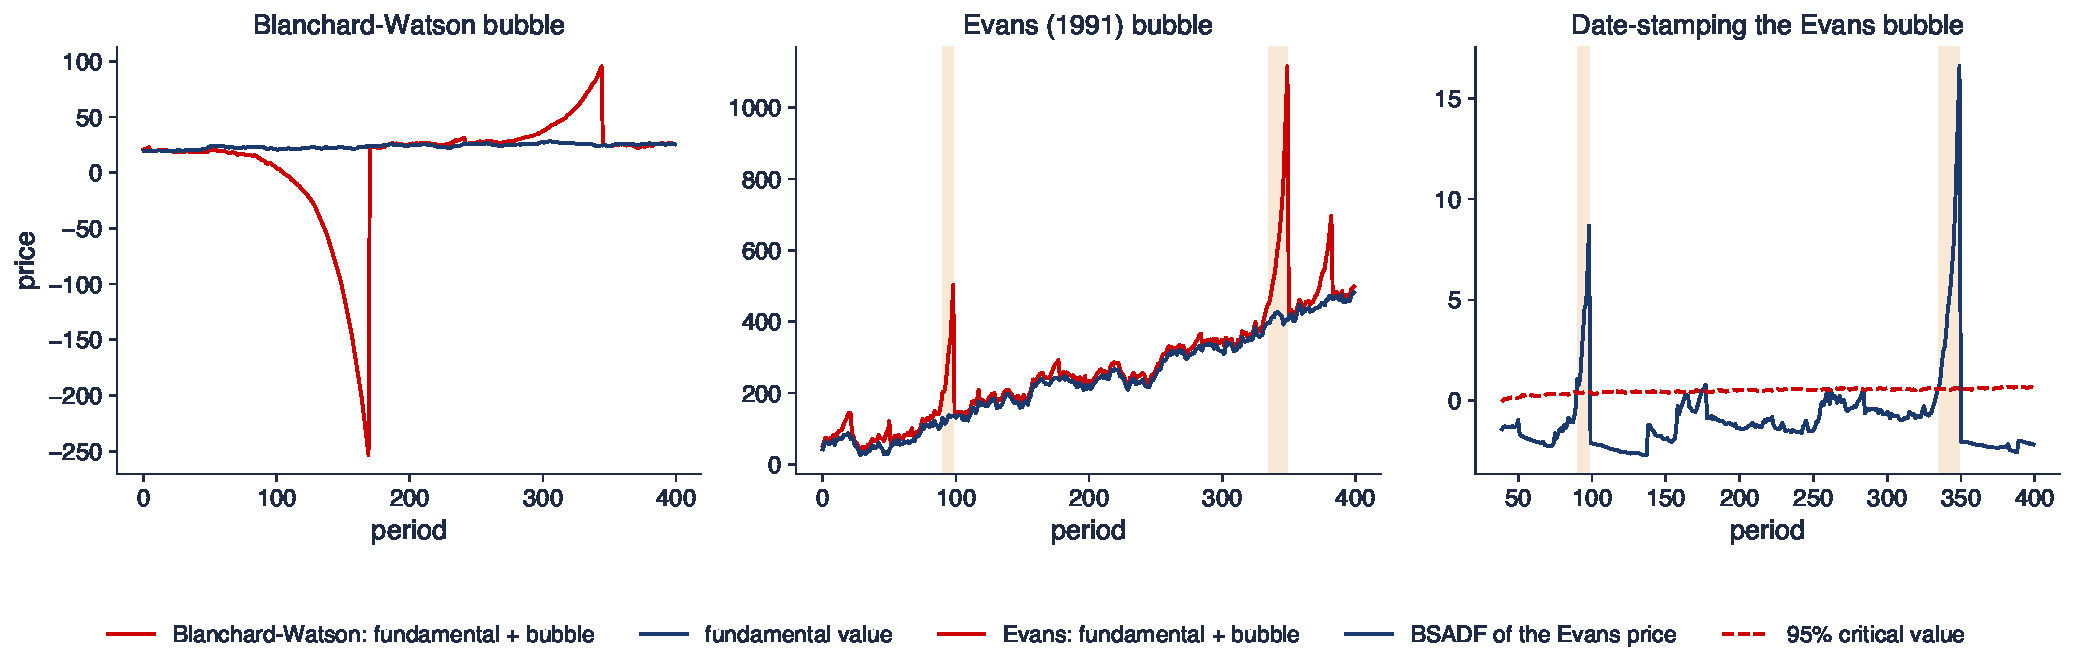
\includegraphics[width=0.97\textwidth,height=0.56\textheight,keepaspectratio]{ats_ch16_rational.pdf}
\end{center}
\vspace{-0.25cm}
\begin{itemize}
    \item Left: Blanchard--Watson, $r = 0.02$, $\pi = 0.98$; middle: Evans bubble times 20 on the fundamental of the worked example ($r = 0.05$, $\alpha = 1$, $\delta = 0.5$, $\pi = 0.85$); right: BSADF of the Evans price against its pointwise 95\% critical value (2\,000 Monte Carlo paths)
    \item Whole-sample ADF $\ensuremath{-}2.81$ (95\% critical value $\ensuremath{-}0.07$); SADF $6.80$ ($1.45$); GSADF $16.58$ ($2.18$); 2 dated episodes
\end{itemize}
\quantlet{ATS\_ch16\_rational\_bubbles}{\qlurl{ATS_ch16_rational_bubbles}}
\end{frame}

\begin{frame}{Interpreting the simulated bubbles}
\itemsize{\small}
\begin{itemize}
    \item The Blanchard--Watson path restarts below zero after a burst and then explodes downwards: exactly the negative bubble that Diba and Grossman exclude
    \item The Evans price looks like its fundamental most of the time; the whole-sample ADF ($\ensuremath{-}2.81$) is even below its 95\% critical value: Evans' pitfall in one number
    \item The window statistics see the large expansions: GSADF $16.58$ against $2.18$; the BSADF sequence crosses its critical value only in the long runs
    \item The minimum-duration rule ($6$ consecutive exceedances) keeps 2 episodes and drops the short bursts: power is traded for fewer false alarms
\end{itemize}
\end{frame}

\begin{frame}{Recap: rational bubbles}
\itemsize{\small}
\begin{itemize}
    \item Price = fundamental + bubble, with $\E_t B_{t+1} = (1 + r)B_t$: a bubble is an explosive autoregressive component
    \item Diba--Grossman: bubbles cannot be negative and cannot start later; they can only grow or burst
    \item Evans: periodic collapses hide the bubble from whole-sample tests; recursive window tests restore the power
    \item Every bubble test is a joint test with the model of the fundamental (a constant $r$, observed dividends or rents)
\end{itemize}
\end{frame}


%=============================================================================
\section{Explosive autoregressions}
%=============================================================================

\begin{frame}{Three regimes of the AR(1) estimator (1/2)}
\itemsize{\small}
{\renewcommand{\arraystretch}{2.0}\begin{center}
\footnotesize
\begin{tabular}{@{}lll@{}}
\toprule
\textbf{Root} & \textbf{Rate and limit of} $\hat\rho - \rho$ & \textbf{Invariance} \\
\midrule
$|\rho| < 1$ & $\sqrt n(\hat\rho - \rho) \Rightarrow N(0, 1 - \rho^2)$ & yes (CLT) \\
$\rho = 1$ & $n(\hat\rho - 1) \Rightarrow \int_0^1 W\,dW \big/ \int_0^1 W^2$ & yes (FCLT) \\
$\rho = 1 + c/k_n$, $k_n \to \infty$, $k_n = o(n)$ & $\dfrac{k_n\rho_n^{\,n}}{2c}(\hat\rho - \rho_n) \Rightarrow \mathcal C$ & yes \refPM{} \\
$|\rho| > 1$ fixed & $\dfrac{\rho^n}{\rho^2 - 1}(\hat\rho - \rho) \Rightarrow \mathcal C$ & only Gaussian errors \refWhi; \refAnd{} \\
\bottomrule
\end{tabular}
\end{center}
}\begin{itemize}
    \item Model: $y_t = \rho y_{t-1} + u_t$, $y_0 = 0$, $u_t$ i.i.d.\ $(0, \sigma^2)$; $\hat\rho$: OLS without intercept
    \begin{itemize}
        \item $n$: sample size; $W$: a standard Brownian motion; $\mathcal C$: the standard Cauchy law; $\Rightarrow$: convergence in distribution
        \item CLT/FCLT: (functional) central limit theorem
    \end{itemize}
\end{itemize}
\end{frame}

\begin{frame}{Three regimes of the AR(1) estimator (2/2)}
\itemsize{\small}
\begin{itemize}
    \item Mildly explosive root: $\rho_n = 1 + c/k_n$
    \begin{itemize}
        \item $c > 0$, and $k_n \to \infty$ more slowly than $n$: $k_n = o(n)$, i.e.\ $k_n/n \to 0$
        \item the Cauchy limit is derived in the \atsapplink{atsapp1}{atssrc1}{Appendix} % applink: the mildly explosive Cauchy limit
    \end{itemize}
    \item The rate grows from $\sqrt n$ to $n$ to the exponential $\rho^n$
    \begin{itemize}
        \item the further from unity, the faster we learn $\rho$
        \item unit roots: \atschlink{https://danpele.github.io/Advanced-Time-Series/EN/Courses/chapter2_structural_breaks_nonlinear_models.pdf}{Chapter 2} and \refHam, Chapter 17
    \end{itemize}
    \item Mildly explosive roots are the realistic case for bubbles
    \begin{itemize}
        \item faster than any local-to-unity root $1 + c/n$
        \item slower than any fixed explosive root
        \item their limit theory is invariant to the error law, unlike the fixed explosive case
    \end{itemize}
\end{itemize}
\end{frame}

\begin{frame}{Worked derivation: where the Cauchy law comes from}
\itemsize{\footnotesize}
\begin{itemize}
    \item $\hat\rho - \rho = \sum_{t} y_{t-1}u_t \big/ \sum_t y_{t-1}^2$ and $y_t = \sum_{j \le t}\rho^{t-j}u_j$
    \item Define $Y_n = \sum_{j=1}^{n}\rho^{-j}u_j$ (dominated by the \textbf{first} shocks) and $X_n = \sum_{j=1}^{n}\rho^{-(n-j)-1}u_j$ (dominated by the \textbf{last} shocks)
    \begin{itemize}
        \item then $\rho^{-n}y_n \approx Y_n$, $\rho^{-2n}\sum_t y_{t-1}^2 \approx Y_n^2/(\rho^2 - 1)$ and $\rho^{-n}\sum_t y_{t-1}u_t \approx X_nY_n$
    \end{itemize}
    \item Hence $\dfrac{\rho^n}{\rho^2 - 1}(\hat\rho - \rho) \approx \dfrac{X_n}{Y_n}$
    \begin{itemize}
        \item $X_n$ and $Y_n$ use disjoint blocks of shocks asymptotically: independent, with equal variances $\sigma^2/(\rho^2 - 1)$
        \item \textbf{fixed} $\rho$: each sum is dominated by a few shocks; it is Gaussian only if the $u_j$ are Gaussian, so the ratio is Cauchy only then \refAnd
        \item \textbf{mildly explosive} $\rho_n$: about $k_n \to \infty$ shocks enter each sum with comparable weights, a CLT applies, and $X_n/Y_n \Rightarrow \mathcal C$ for any i.i.d.\ errors with finite variance \refPM
    \end{itemize}
    \item Pivotal inference: the 95\% interval $\hat\rho \pm (\hat\rho^2 - 1)\hat\rho^{-n}\tan(0.475\pi)$, with $\tan(0.475\pi) \approx 12.71$, replaces $\rho$ by $\hat\rho$ in the norming factor
\end{itemize}
\end{frame}

\begin{frame}{Cauchy limits in finite samples}
\itemsize{\footnotesize}
\begin{center}
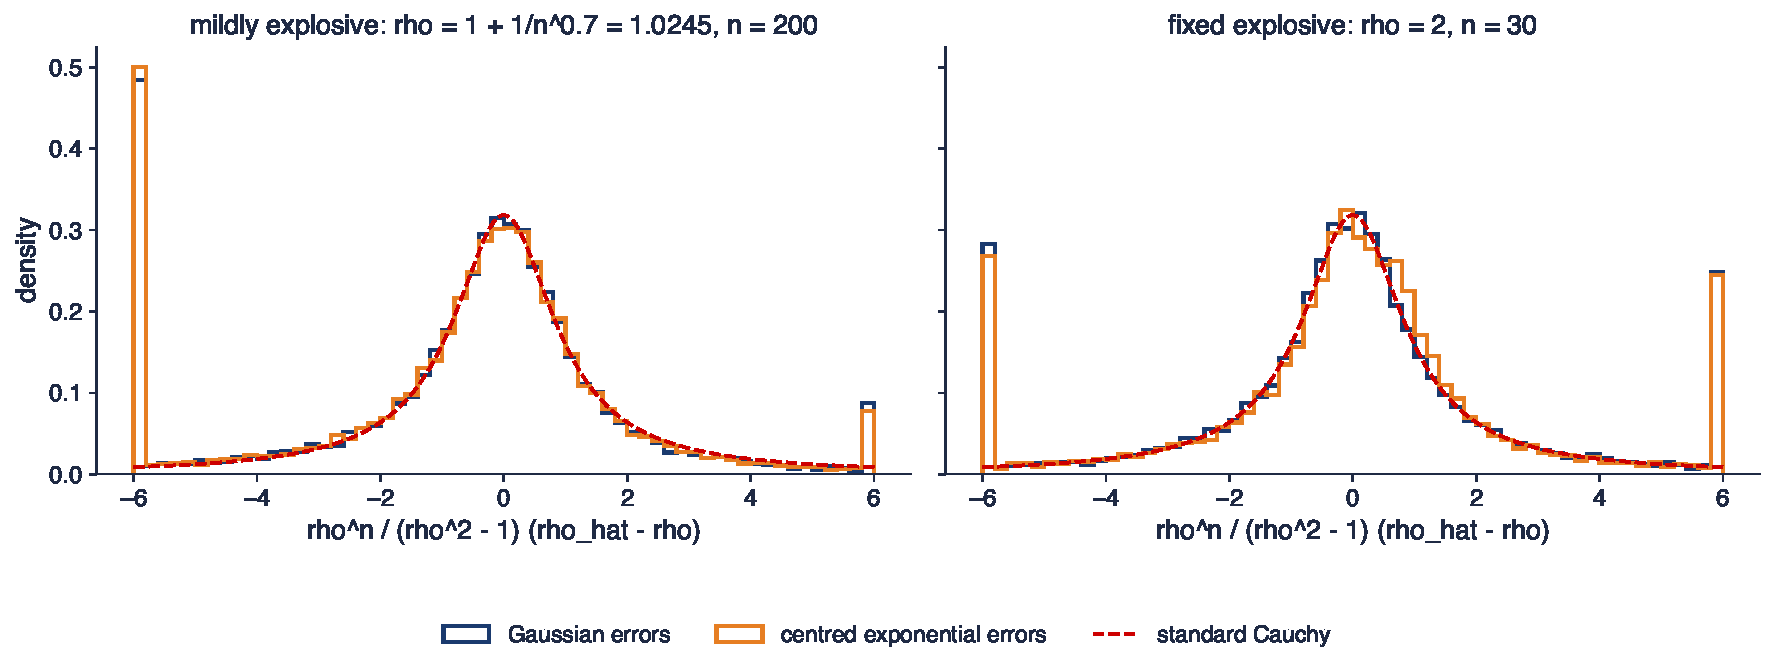
\includegraphics[width=0.97\textwidth,height=0.55\textheight,keepaspectratio]{ats_ch16_asymptotics.pdf}
\end{center}
\vspace{-0.25cm}
\begin{itemize}
    \item 20\,000 samples; normalised error $\rho^n(\hat\rho - \rho)/(\rho^2 - 1)$ with Gaussian and centred exponential errors (skewed), against the Cauchy density
    \item Kolmogorov--Smirnov distance to Cauchy: mild, $n = 200$: 0.060 and 0.062; $n = 2000$ ($\rho = 1.0049$): 0.011 ($p$ = 0.620) and 0.007 ($p$ = 0.945); fixed $\rho = 2$: 0.007 ($p$ = 0.263) and 0.025 ($p$ $<$ 0.001)
\end{itemize}
\quantlet{ATS\_ch16\_explosive\_asymptotics}{\qlurl{ATS_ch16_explosive_asymptotics}}
\end{frame}

\begin{frame}{Interpreting the Cauchy limits}
\itemsize{\small}
\begin{itemize}
    \item Fixed root: with Gaussian errors the Cauchy law fits ($p$ = 0.263); with skewed errors it is rejected ($p$ $<$ 0.001): no invariance principle, as Anderson showed
    \item Mildly explosive root: at $n = 2000$ both error laws give the Cauchy law; at $n = 200$ ($k_n = 40.8$) the approximation is still rough for both: the CLT inside $X_n$ and $Y_n$ needs many effective shocks
    \item Coverage of the 95\% Cauchy interval: 97.0\% and 97.2\% ($n = 200$), 95.0\% and 94.7\% ($n = 2000$): conservative in small samples, accurate in large ones
    \item For bubble tests this is good news: the explosive alternative is learned at an exponential rate, so the window statistics diverge fast once a window sits inside a bubble
\end{itemize}
\end{frame}

\begin{frame}{From limit theory to bubble tests}
\itemsize{\small}
\begin{itemize}
    \item Under a mildly explosive alternative the ADF $t$-statistic diverges to $+\infty$: right-tailed tests are \textbf{consistent} \refPSYb
    \item Levels against logs: a rational bubble is explosive in the \textbf{level}; in logs a pure bubble path $\ln B_0 + t\ln(1 + r)$ is a linear trend
    \begin{itemize}
        \item $\ln(F_t + B_t)$ \textbf{accelerates} while the bubble share rises: log-price tests target accelerating log prices, which is what PWY and PSY test in practice
    \end{itemize}
    \item Specification matters: the intercept, a weak drift $dT^{-\eta}$ ($\eta > 1/2$) in the null, and the lag order change the null limit and the size \refPSYs
    \item Collapses: a sudden fall is a mildly \textbf{integrated} or stationary phase after the explosive one; \refPSi{} date the implosion with a reverse regression
\end{itemize}
\end{frame}

\begin{frame}{Recap: explosive autoregressions}
\itemsize{\small}
\begin{itemize}
    \item Explosive roots are learned at rate $\rho^n$; the limit is Cauchy, a ratio of two independent normals built from the first and the last shocks
    \item Fixed explosive roots have no invariance principle; mildly explosive roots do, which makes them the working model for bubbles
    \item The Cauchy interval for $\rho$ is pivotal but needs large samples; right-tailed tests are consistent against mildly explosive alternatives
\end{itemize}
\end{frame}


%=============================================================================
\section{Recursive tests: theory and size}
%=============================================================================

\begin{frame}{The recursive statistics (1/2)}
\itemsize{\small}
\begin{itemize}
    \item \textbf{Window regression} on the log price $y_t$, over the sample fractions $[r_1, r_2]$ \[ \Delta y_t = a + \delta y_{t-1} + \sum_{j=1}^{k}\phi_j\Delta y_{t-j} + e_t, \qquad t = \lfloor r_1T\rfloor, \dots, \lfloor r_2T\rfloor \]
    \begin{itemize}
        \item $\Delta y_t = y_t - y_{t-1}$; $a$: intercept; $\delta$: the coefficient tested; $\phi_j$: coefficients of $k$ lagged differences; $e_t$: error; $T$: sample size; $\lfloor\cdot\rfloor$: integer part
        \item $\mathrm{ADF}_{r_1}^{r_2}$: the $t$-statistic of $\delta$ on this window
    \end{itemize}
    \item $H_0$: $\delta = 0$ (unit root) against $H_1$: $\delta > 0$ (explosive): a \textbf{right-tailed} test
    \begin{itemize}
        \item minimum window fraction $r_0 = 0.01 + 1.8/\sqrt T$
    \end{itemize}
    \item \textbf{Suprema} over windows \refPWY, \refPSYa{} \[ \mathrm{SADF} = \sup_{r_2 \in [r_0, 1]}\mathrm{ADF}_0^{r_2}, \quad \mathrm{BSADF}_{r_2} = \sup_{r_1 \in [0, r_2 - r_0]}\mathrm{ADF}_{r_1}^{r_2}, \quad \mathrm{GSADF} = \sup_{r_2}\mathrm{BSADF}_{r_2} \]
    \begin{itemize}
        \item SADF: windows starting at the first observation; BSADF: all windows ending at $r_2$ (used to date); GSADF: all windows
    \end{itemize}
\end{itemize}
\end{frame}

\begin{frame}{The recursive statistics (2/2)}
\itemsize{\small}
\begin{itemize}
    \item Null limit (PSY, Theorem 1), with $r_w = r_2 - r_1$ and integrals over $[r_1, r_2]$: \[ \mathrm{ADF}_{r_1}^{r_2} \Rightarrow \dfrac{\frac12 r_w\left[W(r_2)^2 - W(r_1)^2 - r_w\right] - \int W\,dr\,\left[W(r_2) - W(r_1)\right]}{r_w^{1/2}\left\{r_w\int W^2dr - \left(\int W\,dr\right)^2\right\}^{1/2}} \]
    \begin{itemize}
        \item $W$: a standard Brownian motion; $\Rightarrow$: convergence in distribution as $T \to \infty$
        \item pivotal: free of $\sigma$ and of the drift, so critical values depend only on $r_0$, the deterministic terms and $T$ in finite samples
    \end{itemize}
    \item Computation: for $T = 400$ there are 65\,341 window regressions; cumulated cross-products give all of them in $O(T^2)$ operations
\end{itemize}
\end{frame}

\begin{frame}{Null distributions and critical values}
\itemsize{\footnotesize}
\begin{center}
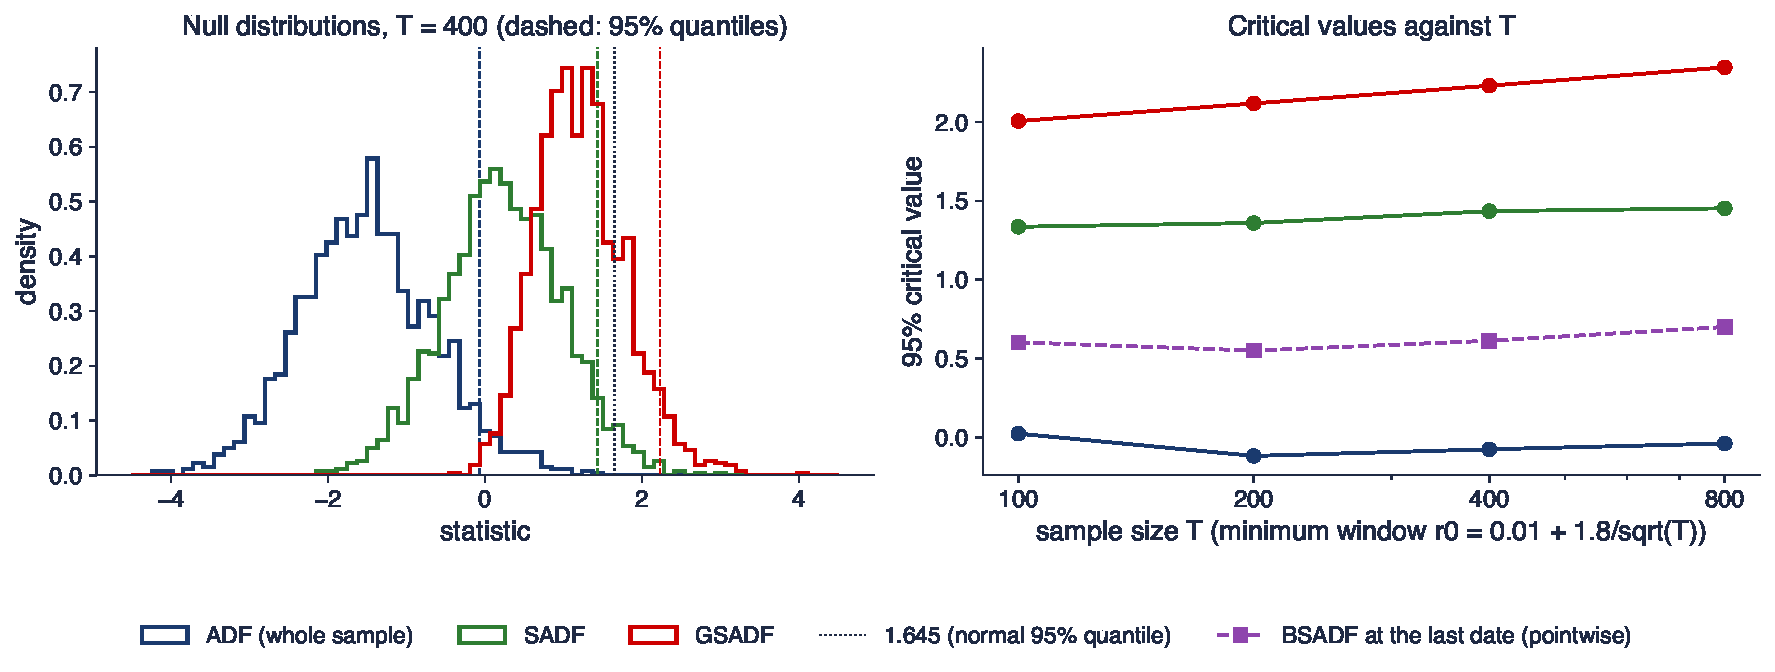
\includegraphics[width=0.97\textwidth,height=0.65\textheight,keepaspectratio]{ats_ch16_null.pdf}
\end{center}
\vspace{-0.25cm}
\begin{itemize}
    \item Null model $y_t = T^{-1} + y_{t-1} + e_t$, $e_t \sim N(0, 1)$, no lags; 95\% critical values at $T = 100, 200, 400, 800$: SADF 1.34, 1.36, 1.43, 1.45; GSADF 2.01, 2.12, 2.23, 2.35
\end{itemize}
\quantlet{ATS\_ch16\_recursive\_tests}{\qlurl{ATS_ch16_recursive_tests}}
\end{frame}

\begin{frame}{Interpreting the null distributions}
\itemsize{\small}
\begin{itemize}
    \item The whole-sample ADF has a negative 95\% quantile (\ensuremath{-}0.07 at $T = 400$): using 1.645 would almost never reject, the right tail of the Dickey--Fuller law is short
    \item Each supremum shifts the distribution to the right: SADF searches over end points, GSADF over start and end points; the GSADF bar is the price of the search
    \item The GSADF critical value rises with $T$ (2.01 to 2.35) although $r_0$ falls: more windows, a larger maximum; tabulate critical values for your own $T$, $r_0$ and lag order
    \item The pointwise 95\% quantile of BSADF at the last date (0.61 at $T = 400$) is far below the GSADF one: a single date is tested at 5\%, the whole path is not
\end{itemize}
\end{frame}

\begin{frame}{Changing volatility and the wild bootstrap}
\itemsize{\small}
\begin{itemize}
    \item The pivotal limit assumes homoskedastic shocks; with a volatility shift the limit involves the variance profile, and Monte Carlo critical values give the wrong size \refHLST
    \begin{itemize}
        \item a late rise in volatility looks like acceleration; a fall in volatility makes the test conservative
    \end{itemize}
    \item \textbf{Wild bootstrap} \refPS: fit the null $\Delta y_t = \mu + \sum_j\phi_j\Delta y_{t-j} + e_t$, draw Rademacher signs $w_t = \pm 1$, build $\Delta y^*_t = \sum_j\hat\phi_j\Delta y^*_{t-j} + w_t\hat e_t$, cumulate, recompute the statistics
    \begin{itemize}
        \item the bootstrap series has a unit root by construction and the \textbf{same volatility pattern} $|\hat e_t|$ as the data
        \item critical values: pointwise quantiles of BSADF, the quantile of the maximum (GSADF), or the quantile of the maximum over a moving window
    \end{itemize}
    \item Alternatives for non-stationary volatility: weighted and sign-based statistics \refHLZ; end-of-sample tests \refAHLT
\end{itemize}
\end{frame}

\begin{frame}{Many dates, one false alarm}
\itemsize{\small}
\begin{itemize}
    \item Date-stamping compares $\mathrm{BSADF}_{r_2}$ with a \textbf{pointwise} critical value at every date: each date has a 5\% false-alarm chance, but a sample has hundreds of dates
    \begin{itemize}
        \item BSADF is highly autocorrelated in $r_2$, so false alarms come in runs: the minimum-duration rule removes the shortest runs only
    \end{itemize}
    \item \textbf{Family-wise error rate} (FWER): the probability of at least one false alarm over a set of dates
    \begin{itemize}
        \item over the whole sample: compare BSADF with the 95\% quantile of its maximum, i.e.\ the GSADF critical value
        \item over a moving window of $\tau_b$ dates \refPS: the 95\% bootstrap quantile of $\max_{s \in (t - \tau_b, t]}\mathrm{BSADF}_s$; here $\tau_b = 52$ weeks
    \end{itemize}
    \item Asymptotically, consistent dating needs critical values that diverge slowly, so that the false-alarm probability vanishes \refPSYb; in practice a fixed 5\% at every date is used, and its cost must be measured
\end{itemize}
\end{frame}

\begin{frame}{Size under changing volatility and across dates}
\itemsize{\footnotesize}
\begin{center}
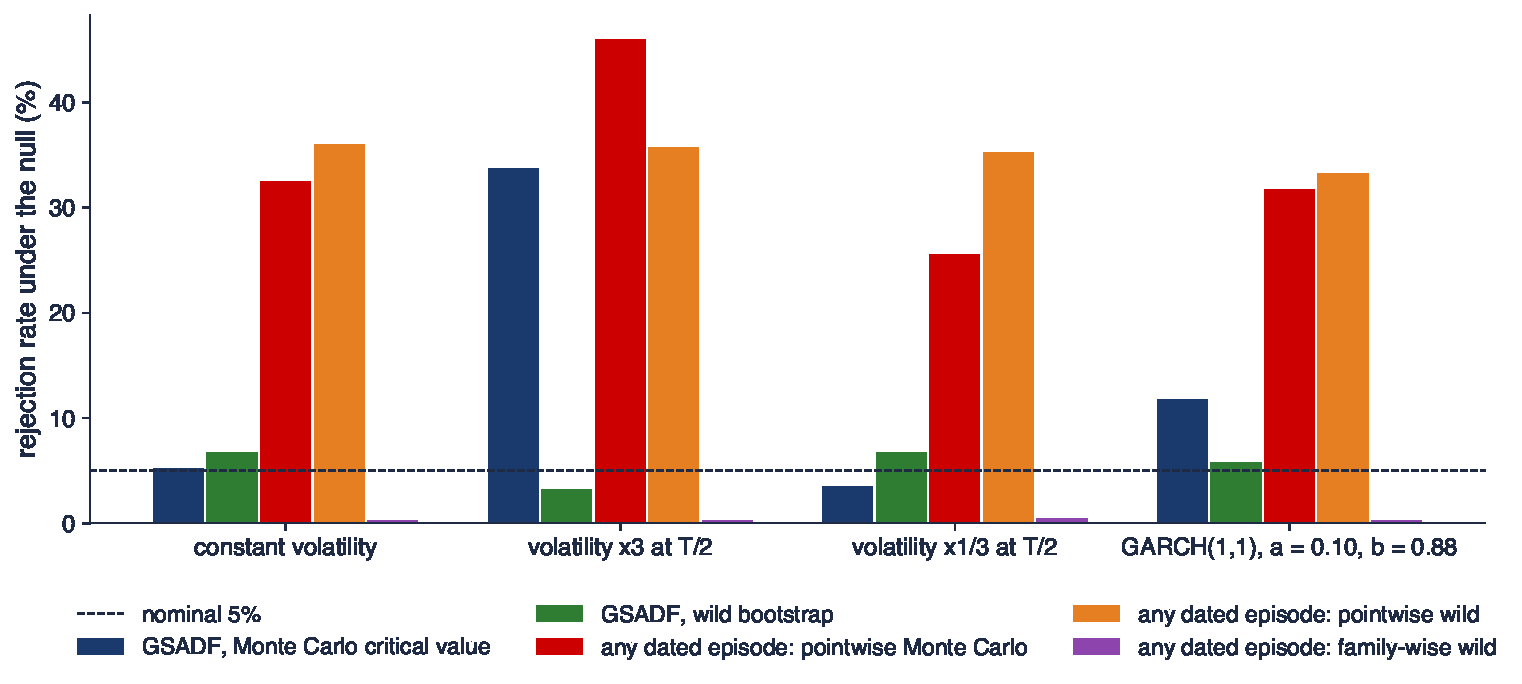
\includegraphics[width=0.97\textwidth,height=0.65\textheight,keepaspectratio]{ats_ch16_size.pdf}
\end{center}
\vspace{-0.25cm}
\begin{itemize}
    \item 400 null paths of $T = 200$ per design, each with its own wild bootstrap (199 draws); a dated episode needs 6 consecutive exceedances; nominal level 5\%
\end{itemize}
\quantlet{ATS\_ch16\_size\_wild\_bootstrap}{\qlurl{ATS_ch16_size_wild_bootstrap}}
\end{frame}

\begin{frame}{Interpreting the size study}
\itemsize{\small}
\begin{itemize}
    \item GSADF with Monte Carlo critical values: 5.2\% with constant volatility, 33.8\% after a late tripling, 11.8\% under GARCH; the wild bootstrap gives 6.8\%, 3.2\% and 5.8\%
    \item Pointwise dating finds at least one episode in 32.5\% (Monte Carlo) and 36.0\% (wild) of paths \textbf{without any bubble}, even with constant volatility
    \item With the family-wise threshold over the whole sample, false episodes fall to 0.2\%--0.5\%: below 5\%, because an episode also needs 6 consecutive exceedances; the cost is power and later dates
    \item Lesson: report which error rate a dated episode controls; a 5\% pointwise test on every week is not a 5\% test of the sample
\end{itemize}
\end{frame}

\begin{frame}{Recap: recursive tests}
\itemsize{\small}
\begin{itemize}
    \item SADF, GSADF and BSADF are suprema of window ADF statistics with a pivotal null limit; critical values must match $T$, $r_0$, the deterministic terms and the lags
    \item Changing volatility distorts the size; the wild bootstrap keeps the volatility pattern and restores it
    \item Pointwise dating has a high false-episode rate over a sample; family-wise thresholds control it at the cost of power
\end{itemize}
\end{frame}


%=============================================================================
\section{Date-stamping and early warning}
%=============================================================================

\begin{frame}{Date-stamping rules and their accuracy}
\itemsize{\small}
\begin{itemize}
    \item \textbf{Origination and termination} \refPSYa: the first date where BSADF exceeds its critical value, and the first later date where it falls back below \[ \hat r_e = \inf\{r_2 \ge r_0: \mathrm{BSADF}_{r_2} > cv_{r_2}\}, \qquad \hat r_f = \inf\{r_2 \ge \hat r_e + \delta\ln(T)/T: \mathrm{BSADF}_{r_2} < cv_{r_2}\} \]
    \begin{itemize}
        \item $cv_{r_2}$: the pointwise 95\% critical value at $r_2$; $\delta\ln(T)/T$: a minimum duration (with $\delta$ a tuning constant)
        \item here: an episode is a run of at least $\lceil\ln T\rceil$ consecutive exceedances, dated from the first to the last one (as in \texttt{exuber} \refVPM)
    \end{itemize}
    \item In real time an episode is \textbf{confirmed} only after the minimum duration: the alarm date is the start plus $\lceil\ln T\rceil - 1$
    \item Consistency of $(\hat r_e, \hat r_f)$ holds for mildly explosive bubbles of fixed fractional duration \refPSYb
    \begin{itemize}
        \item the start is dated late, because a window must first accumulate explosive observations
        \item improved start and end estimators that use the whole bubble period: \refHLS
    \end{itemize}
\end{itemize}
\end{frame}

\begin{frame}{Date-stamping: design of the experiment}
\itemsize{\small}
\begin{itemize}
    \item Simulated paths: random walk from $y_0 = 100$, then an explosive phase, a collapse, and a random walk again
    \begin{itemize}
        \item explosive phase $y_t = \rho y_{t-1} + e_t$, $\rho > 1$, on periods 200--260; $e_t$: Normal noise
        \item collapse to the pre-bubble level at the end of the explosive phase
        \item $T = 400$, 1\,000 paths for each value of $\rho$
    \end{itemize}
    \item Questions: how often is the bubble found, how late is its start dated, how often is a false episode dated before it?
\end{itemize}
\end{frame}

\begin{frame}{How late is the start dated?}
\itemsize{\footnotesize}
\begin{center}
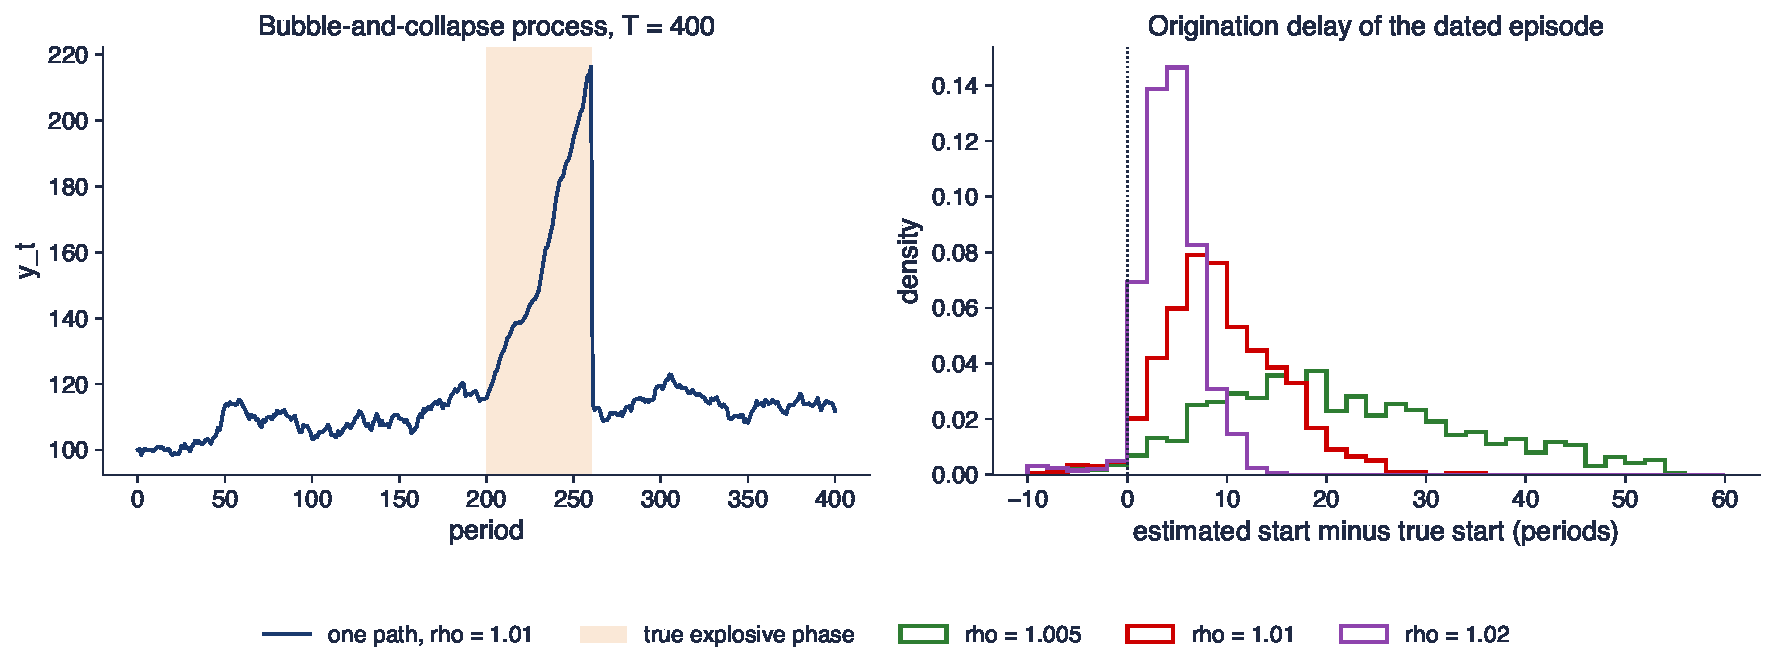
\includegraphics[width=0.97\textwidth,height=0.65\textheight,keepaspectratio]{ats_ch16_dating.pdf}
\end{center}
\vspace{-0.25cm}
\begin{itemize}
    \item Delay of the first dated exceedance after the true start (periods); pointwise 95\% Monte Carlo critical values; growth over the bubble $\rho^{60}$: 1.35, 1.82 and 3.28
\end{itemize}
\quantlet{ATS\_ch16\_date\_stamping}{\qlurl{ATS_ch16_date_stamping}}
\end{frame}

\begin{frame}{Interpreting the date-stamping experiment}
\itemsize{\small}
\begin{itemize}
    \item Detection rates 94.9\%, 100.0\% and 100.0\% for $\rho = 1.005, 1.01, 1.02$: a bubble of 60 periods is almost always found
    \item Median start delays 19, 8 and 4 periods (interquartile ranges 11--29, 5--13, 2--6); confirmation adds 6 $-$ 1 periods: medians 24, 13, 9
    \item For the slowest bubble the alarm comes after about a third of its life: a detector of \textbf{ongoing} exuberance, not of its birth
    \item In 26\%--31\% of paths a false episode is dated \textbf{before} the bubble starts: the multiplicity of the previous section, now inside a true-bubble design
\end{itemize}
\end{frame}

\begin{frame}{Real-time monitoring (1/2)}
\itemsize{\small}
\begin{itemize}
    \item Monitoring: a training sample of $n$ observations without a bubble, then a decision at each new date $t > n$; the error rate is over the \textbf{whole} monitoring horizon \refCSW
    \item \textbf{CUSUM} of returns: cumulated deviations of the new returns from the training mean, in units of the training volatility \[ S_t = \sum_{j=n+1}^{t}\frac{r_j - \bar r_n}{\hat\sigma_n\sqrt n}, \qquad \text{alarm when}\ S_t > b_t = \sqrt{\tfrac{t - n}{n}\cdot\tfrac{t}{n}\left[a^2 + \ln\tfrac{t}{t - n}\right]} \]
    \begin{itemize}
        \item $r_j$: return of period $j$; $\bar r_n$, $\hat\sigma_n$: mean and standard deviation of the training returns; $b_t$: the boundary, which widens with $t$; $a$: a constant that sets the error rate
    \end{itemize}
    \item Error rate over the whole horizon (proof in the \atsapplink{atsapp2}{atssrc2}{Appendix})
    \begin{itemize}
        \item $\Pr\{S_t > b_t$ for some $t\} \to 1 - \Phi(a) + a\varphi(a)$; $\Phi$, $\varphi$: standard Normal distribution and density functions
        \item 5\% gives $a = 2.50$, $a^2 = 6.25$
    \end{itemize}
\end{itemize}
\end{frame}

\begin{frame}{Real-time monitoring (2/2)}
\itemsize{\small}
\begin{itemize}
    \item Simulated size, $n = 100$, horizon $5n$, 2\,000 paths
    \begin{itemize}
        \item 3.5\% with i.i.d.\ returns, 6.0\% with GARCH returns
    \end{itemize}
    \item \refHB{} compare bubble tests and monitoring schemes and recommend monitoring of this kind for real time
    \begin{itemize}
        \item \refAHLST{} give monitoring statistics with controlled size for explosive bubbles
    \end{itemize}
    \item BSADF in real time is also a monitor: $\mathrm{BSADF}_t$ uses only data up to $t$, but its pointwise critical values do not control the error over the horizon
\end{itemize}
\end{frame}

\begin{frame}{Monitoring the Nasdaq 100 and Bitcoin}
\itemsize{\footnotesize}
\begin{center}
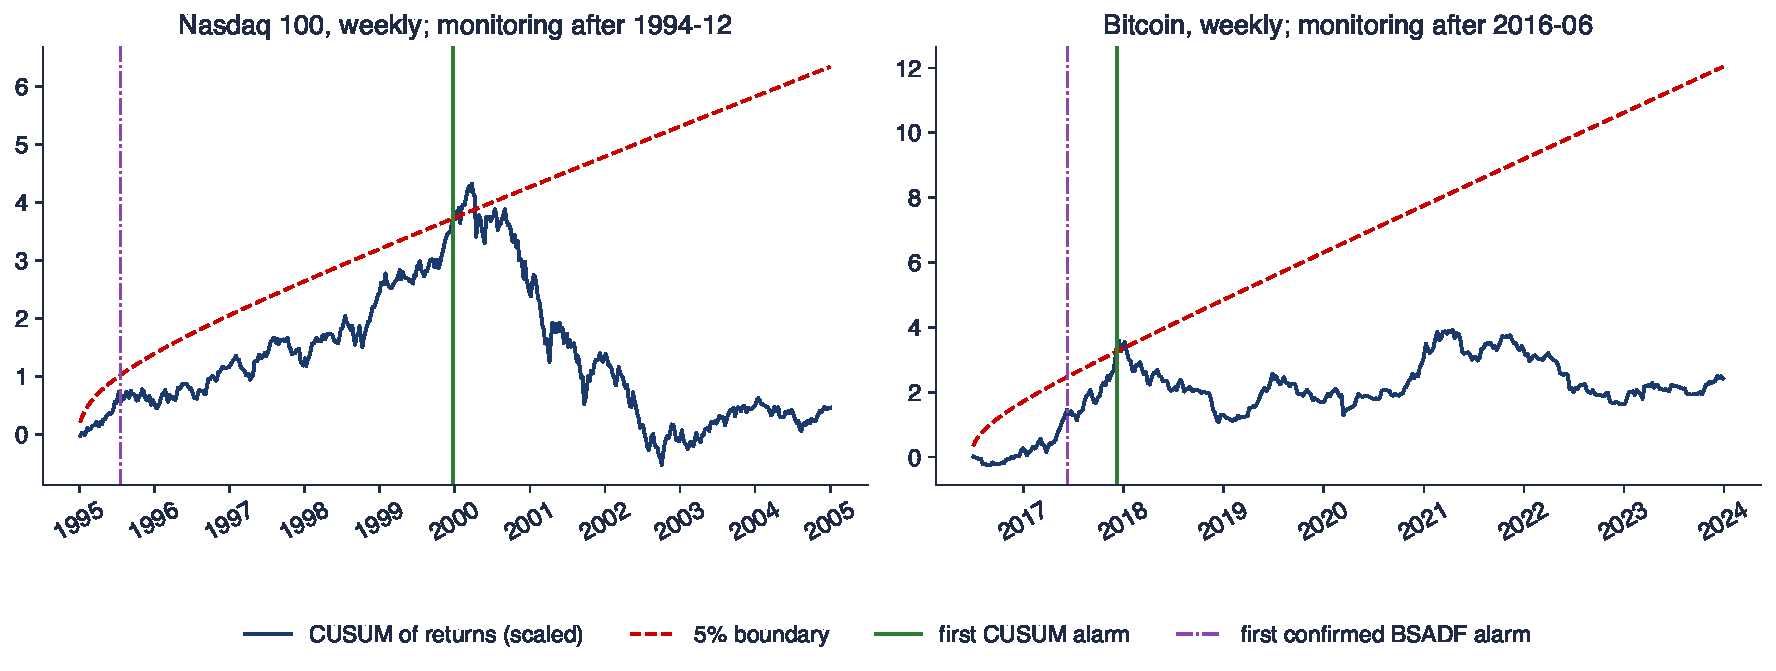
\includegraphics[width=0.97\textwidth,height=0.65\textheight,keepaspectratio]{ats_ch16_monitor.pdf}
\end{center}
\vspace{-0.25cm}
\begin{itemize}
    \item Weekly log returns; training: 1990--1994 (Nasdaq 100, $n = 260$) and September 2014 -- June 2016 (Bitcoin, $n = 92$); BSADF with pointwise Monte Carlo critical values
\end{itemize}
\quantlet{ATS\_ch16\_monitoring}{\qlurl{ATS_ch16_monitoring}}
\end{frame}

\begin{frame}{Interpreting the monitoring charts}
\itemsize{\small}
\begin{itemize}
    \item Nasdaq 100: the CUSUM alarm comes on 24 December 1999, three months before the peak of 24 March 2000; the first confirmed BSADF alarm after training comes on 21 July 1995, more than four years earlier
    \item Bitcoin: CUSUM on 8 December 2017, at the top of the 2017 run-up; BSADF on 9 June 2017
    \begin{itemize}
        \item the boundary widens with $\sqrt{t\ln t}$, so after 2018 the 2021 rally cannot reach it
    \end{itemize}
    \item CUSUM detects a change in the mean return (persistent acceleration), not explosiveness as such; it is slow, but its size is controlled over the whole horizon
    \item BSADF reacts early and often: an early alarm that is followed by years of further gains is costly to anyone who acts on it
\end{itemize}
\end{frame}

\begin{frame}{Evaluating early warnings honestly}
\itemsize{\small}
\begin{itemize}
    \item Define the \textbf{event} before looking at alarms: here a fall of at least 20\% within 182 days after the date; define the \textbf{alarm} rule and the evaluation dates (every fifth trading day)
    \item Hit rate $H = \Pr(\text{alarm} \mid \text{event})$, false-alarm rate $F = \Pr(\text{alarm} \mid \text{no event})$, base rate $\pi_0 = \Pr(\text{event})$
    \begin{itemize}
        \item \textbf{precision} by Bayes: $\Pr(\text{event} \mid \text{alarm}) = H\pi_0 / [H\pi_0 + F(1 - \pi_0)]$; with $\pi_0 = 5\%$, $H = 80\%$, $F = 20\%$ it is only 17\%
        \item the noise-to-signal ratio $F/H$ of the early-warning literature \refKLR
    \end{itemize}
    \item \textbf{ROC curve}: $(F, H)$ for every threshold of a continuous score; \textbf{AUC} $= \Pr(\text{score of an event date} > \text{score of a non-event date})$; 0.5 means no skill
    \item Overlapping horizons make evaluation dates strongly dependent: intervals for the AUC need a moving-block bootstrap (\atschlink{https://danpele.github.io/Advanced-Time-Series/EN/Courses/chapter0_refresher_inference.pdf}{Chapter 0}), and a few crashes carry the whole sample
\end{itemize}
\end{frame}

\begin{frame}{Recap: date-stamping and early warning}
\itemsize{\small}
\begin{itemize}
    \item BSADF dates the start late (after a run of explosive observations) and confirms it later still; slow bubbles are found after a large part of their life
    \item Monitoring with a boundary controls the error over the whole horizon; pointwise BSADF does not
    \item Evaluate alarms with hit rate, false-alarm rate, precision at the base rate and ROC/AUC, with block-bootstrap intervals
\end{itemize}
\end{frame}


%=============================================================================
\section{Fundamentals against prices}
%=============================================================================

\begin{frame}{Testing the ratio, the price and the fundamental}
\itemsize{\footnotesize}
\begin{columns}[T]
\begin{column}{0.34\textwidth}
\centering
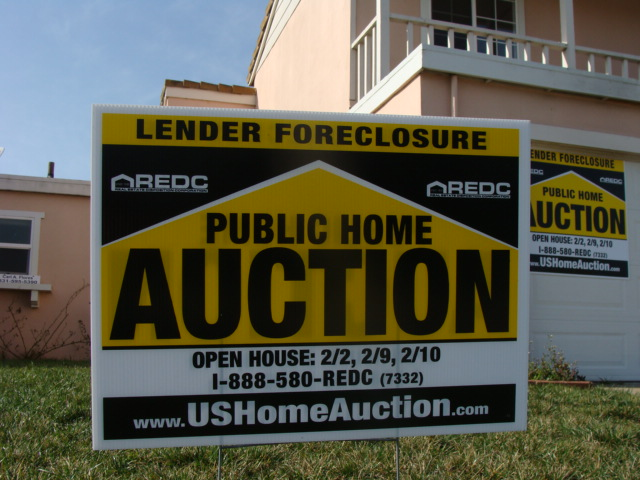
\includegraphics[height=0.36\textheight]{ch16_foreclosure_2008.jpg}\\[1mm]
\imgcap{A foreclosed home in the United States, 2008}
\imgcredit{https://commons.wikimedia.org/wiki/File:Foreclosedhome.JPG}{Photo: Brendel (2008); CC BY-SA 3.0; Wikimedia Commons}
\end{column}
\begin{column}{0.64\textwidth}
\begin{itemize}
    \item Under the present-value model the price-to-rent (or price-dividend) ratio is stationary; an explosive \textbf{ratio} with a non-explosive \textbf{fundamental} points to a bubble
    \item If rents themselves explode, an explosive price is not evidence of a bubble: test both (the logic of \refDGb{} applied with PSY)
    \item Landmarks: \refPY{} date the US price-to-rent exuberance before the subprime crisis; \refPav{} apply GSADF to the international housing panel of the Dallas Fed
    \item Monthly house prices are smoothed (repeat-sales indices, appraisals): their changes are autocorrelated, so the lag order $k$ matters; here $k$ by BIC, up to 6 months
\end{itemize}
\end{column}
\end{columns}
\end{frame}

\begin{frame}{US and Romanian housing: ratio and fundamental}
\itemsize{\footnotesize}
\begin{center}
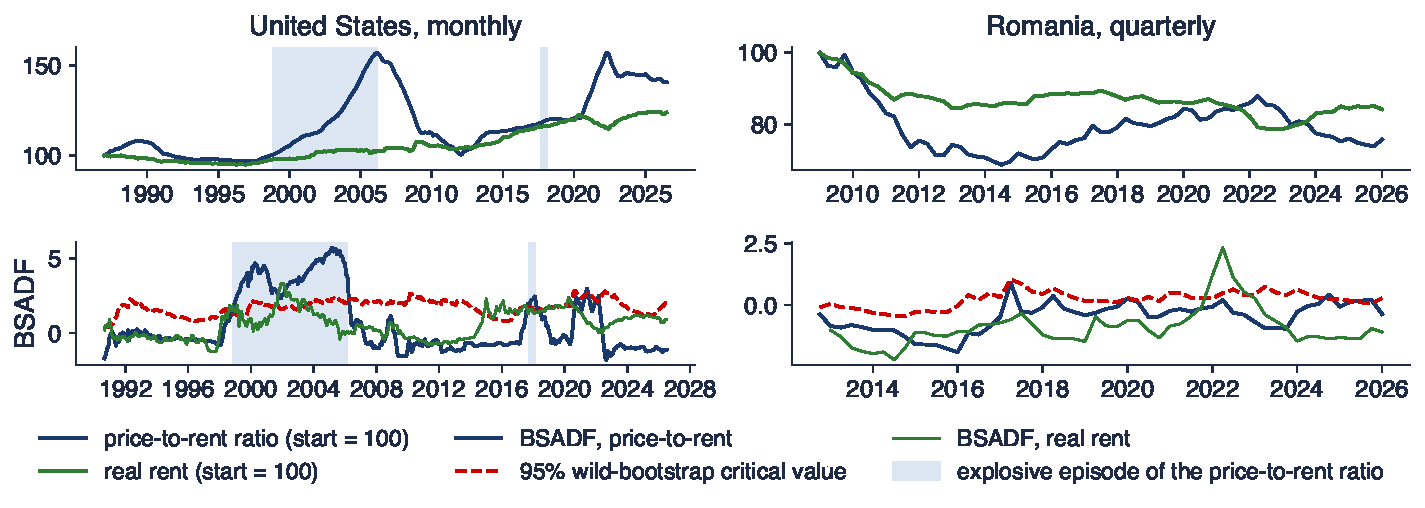
\includegraphics[width=0.97\textwidth,height=0.65\textheight,keepaspectratio]{ats_ch16_housing.pdf}
\end{center}
\vspace{-0.25cm}
\begin{itemize}
    \item Log price-to-rent and log real rent; BSADF with $k$ lags (US ratio $k = 1$, rent $k = 1$) and pointwise 95\% wild-bootstrap critical values (999 draws); shaded: dated episodes of the ratio
\end{itemize}
\quantlet{ATS\_ch16\_housing}{\qlurl{ATS_ch16_housing}}
\end{frame}

\begin{frame}{Interpreting the housing tests}
\itemsize{\footnotesize}
\begin{itemize}
    \item US price-to-rent: GSADF 5.75 against the wild-bootstrap value 4.47; the main episode runs from November 1998 to March 2006, the boom before the subprime crisis found by \refPY
    \item US real rent: GSADF 3.35 against 3.25, with episodes February 1998--March 1999; June 2001--September 2004; September 2014--May 2021; September 2023--April 2026: the fundamental also accelerated, so the 2014--2022 price rise is partly a rent story
    \item US real house price alone: episodes February 2002--March 2006; December 2020--May 2022; the 2020--2022 surge is explosive in the price but not in the ratio, unlike 1998--2006
    \item Romania (quarterly, $T = 68$): GSADF of the ratio 0.91 against 1.38, of the real price 0.88 against 2.11: no explosive episode since 2009; the HICP rent index jumps by 33\% in April 2026, so the sample ends in March 2026
\end{itemize}
\end{frame}

\begin{frame}{Recap: fundamentals against prices}
\itemsize{\small}
\begin{itemize}
    \item Test the ratio and the fundamental separately: an explosive ratio with a calm fundamental is the bubble signature
    \item Smoothed housing indices need lag augmentation and a bootstrap under the AR null; without lags the tests reject almost everywhere
    \item Short samples (Romania since 2009) have little power: no rejection is not evidence of no bubble
\end{itemize}
\end{frame}


%=============================================================================
\section{LPPLS as a competing detector}
%=============================================================================

\begin{frame}{LPPLS in one slide}
\itemsize{\footnotesize}
\begin{columns}[T]
\begin{column}{0.3\textwidth}
\centering

\includegraphics[height=0.36\textheight]{ch16_sornette_2012.jpg}\\[1mm]
\imgcap{Didier Sornette, 2012}
\imgcredit{https://commons.wikimedia.org/wiki/File:Didier_Sornette.jpg}{Photo: Didier Sornette (2012); CC BY-SA 3.0 de; Wikimedia Commons}
\end{column}
\begin{column}{0.68\textwidth}
\begin{itemize}
    \item \refJLS: the log price grows faster than exponentially towards a critical time $t_c$, with oscillations that speed up \[ \ln p(t) = A + B(t_c - t)^m + C_1(t_c - t)^m\cos(\omega\ln(t_c - t)) + C_2(t_c - t)^m\sin(\omega\ln(t_c - t)) \]
    \begin{itemize}
        \item $A$: log price at $t_c$; $B < 0$ and $0 < m < 1$: super-exponential growth; $C_1$, $C_2$: amplitudes of the oscillations; $\omega$: their log-frequency
    \end{itemize}
    \item Two steps \refFS: for given $(t_c, m, \omega)$ the four linear parameters are OLS; minimise the concentrated sum of squares over three nonlinear parameters
    \item Qualified fits: the filter of \refSZ{} (bounds on $m$, $\omega$, $t_c$, number of oscillations, damping, relative error, Lomb test, stationary residuals)
    \item \textbf{Confidence indicator}: the share of qualified fits over many windows ending at the same date (here 29 windows of 50--750 days)
\end{itemize}
\end{column}
\end{columns}
\end{frame}

\begin{frame}{Inference on the critical time}
\itemsize{\small}
\begin{itemize}
    \item The point estimate $\hat t_c$ moves with the window and the data; an \textbf{interval} is needed
    \item \textbf{Profile likelihood}: for each $t_c$, the other parameters are set to their best values; with Gaussian errors \[ \ell(t_c) = -\frac n2\ln\big[\mathrm{SSR}(t_c)/n\big], \qquad \text{95\% interval}: \{t_c: 2[\ell(\hat t_c) - \ell(t_c)] \le \chi^2_{1;0.95} = 3.84\} \]
    \begin{itemize}
        \item $n$: number of days in the window; $\mathrm{SSR}(t_c)$: the smallest sum of squared residuals for this $t_c$
        \item too narrow when residuals are autocorrelated or when nuisance parameters are many
    \end{itemize}
    \item \refFDS: the modified profile likelihood (Barndorff-Nielsen) corrects for the nuisance parameters; intervals for $t_c$ become wider and asymmetric
    \item \refDS{} ask whether the birth or the burst of a bubble is easier to diagnose: the start time is far better constrained by the data than $t_c$
\end{itemize}
\end{frame}

\begin{frame}{Shanghai 2015: indicator and critical time}
\itemsize{\footnotesize}
\begin{center}
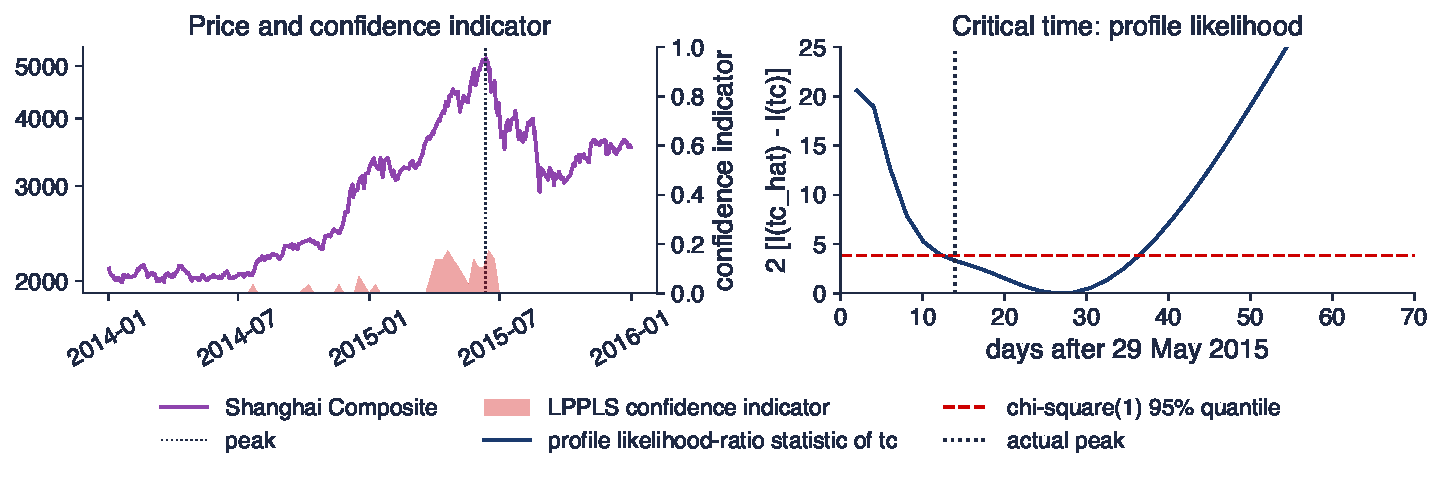
\includegraphics[width=0.97\textwidth,height=0.61\textheight,keepaspectratio]{ats_ch16_lppls.pdf}
\end{center}
\vspace{-0.25cm}
\begin{itemize}
    \item Left: confidence indicator every fifth trading day; right: profile likelihood of $t_c$ for the window from the low of 20 March 2014 to 29 May 2015 (293 days), as in the real-time analysis of \refSha
\end{itemize}
\quantlet{ATS\_ch16\_lppls\_inference}{\qlurl{ATS_ch16_lppls_inference}}
\end{frame}

\begin{frame}{Interpreting the Shanghai fit}
\itemsize{\small}
\begin{itemize}
    \item The fit ending on 29 May 2015 passes the whole filter: $m = 0.41$, $\omega = 6.28$, 5.7 oscillations, damping 1.16; $\hat t_c$ = 24 June 2015
    \item Profile-likelihood interval: 12 June 2015 to 2 July 2015 (20 days); the peak of 12 June 2015 lies at its left edge: a good call that is fragile to the window
    \item The indicator is low: at most 0.17 (on 20 April 2015); few windows qualify at once, so the indicator flags a regime, not a date
    \item One success is an anecdote: the next section counts alarms over decades, with base rates
\end{itemize}
\end{frame}

\begin{frame}{Spectral views of log-periodicity and the critique}
\itemsize{\small}
\begin{itemize}
    \item The oscillation $\cos(\omega\ln(t_c - t))$ is periodic in $\ln(t_c - t)$
    \begin{itemize}
        \item test: the Lomb periodogram of the detrended residual against $\ln(t_c - t)$ \refLom
        \item nonparametric alternative: the $(H, q)$-derivative analysis \refZS
        \item in calendar time its instantaneous frequency is $\omega/[2\pi(t_c - t)]$: oscillations speed up towards $t_c$; the Hilbert transform of the residual gives this phase directly (\atschlink{https://danpele.github.io/Advanced-Time-Series/EN/Courses/chapter11_spectral_wavelet_analysis.pdf}{Chapter 11} for the tools)
    \end{itemize}
    \item Critique
    \begin{itemize}
        \item log-periodic peaks appear in noise after fitting and detrending \refFei
        \item out-of-sample crash calls perform poorly \refBJ; estimation is fragile \refGF
        \item replies on the stochastic formulation, filters and multi-window indicators: \refSWYZ
    \end{itemize}
    \item A fair comparison with PSY uses the same events, dates and error measures: next section
\end{itemize}
\end{frame}

\begin{frame}{Recap: LPPLS}
\itemsize{\small}
\begin{itemize}
    \item LPPLS models super-exponential growth with log-periodic oscillations towards a critical time; the confidence indicator aggregates qualified fits over windows
    \item The critical time needs an interval: profile or modified profile likelihood; the birth of a bubble is easier to pin down than its burst
    \item Spectral tests of log-periodicity are easy to fool; judge LPPLS by its alarms, not by its fits
\end{itemize}
\end{frame}


%=============================================================================
\section{Applications with base rates}
%=============================================================================

\begin{frame}{Five episodes, one protocol}
\itemsize{\footnotesize}
\begin{columns}[T]
\begin{column}{0.34\textwidth}
\centering
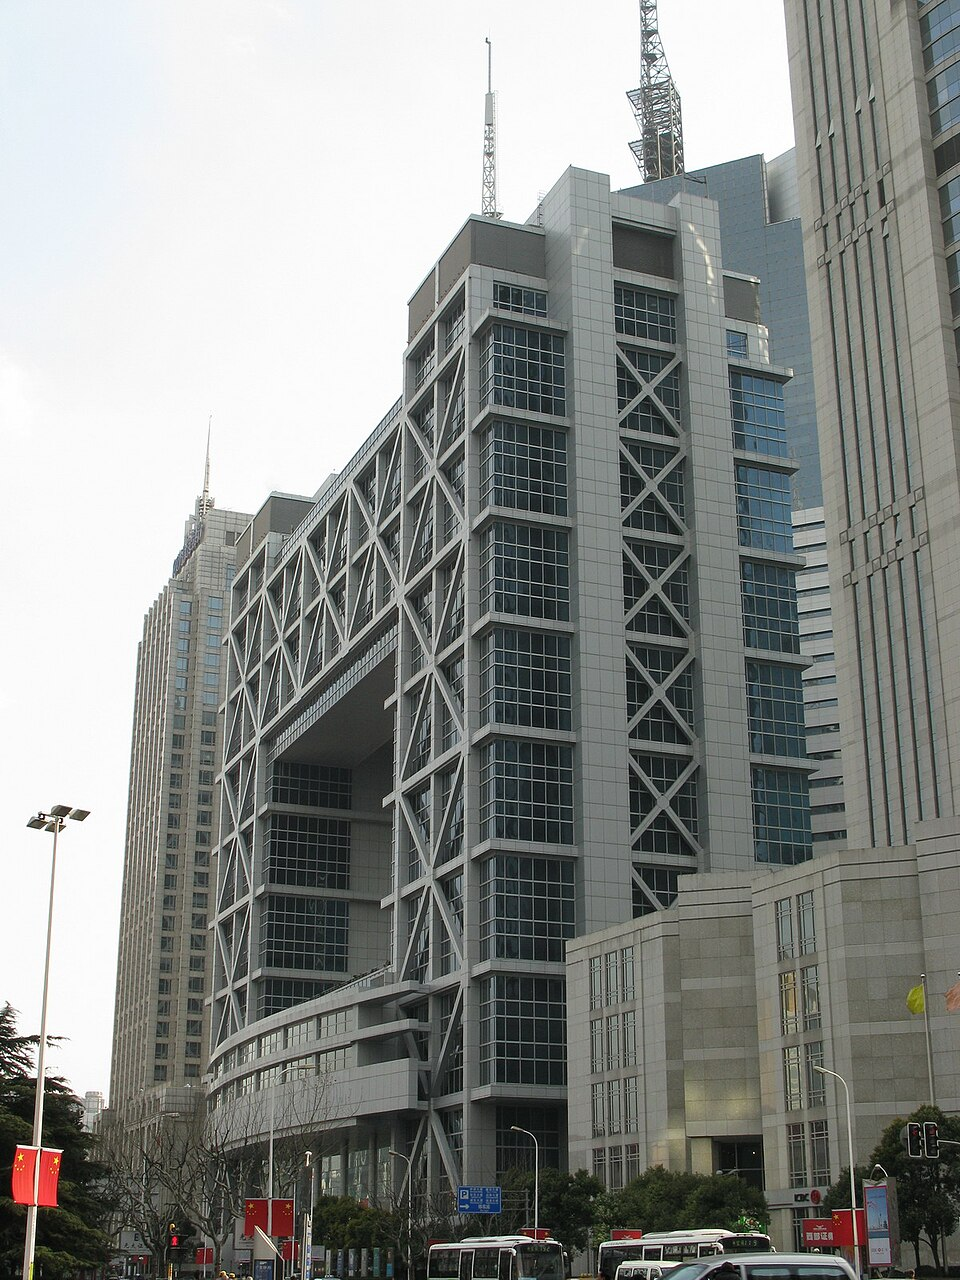
\includegraphics[height=0.4\textheight]{ch16_shanghai_se_2008.jpg}\\[1mm]
\imgcap{Shanghai Stock Exchange, Pudong, 2008}
\imgcredit{https://commons.wikimedia.org/wiki/File:Shanghai_Stock_Exchange_Building.jpg}{Photo: Baycrest (2008); CC BY-SA 2.5; Wikimedia Commons}
\end{column}
\begin{column}{0.64\textwidth}
\begin{itemize}
    \item Weekly log prices (Friday close): S\&P 500 and Nasdaq 100 1990--2004, Shanghai Composite 2010--2018, Bitcoin September 2014 -- 2023, BET 2000--2012
    \item No lags; $r_0 = 0.01 + 1.8/\sqrt T$; minimum duration $\lceil\ln T\rceil$ weeks; Monte Carlo (1000 paths) and wild-bootstrap (499 draws) critical values
    \item Episodes dated with pointwise wild values and with the family-wise wild threshold over 52 weeks; the alarm date is the confirmation date
    \item Case studies: \refPWY{} (Nasdaq), \refPSYa{} (S\&P 500), \refSha{} (Shanghai), \refGDS{} (Bitcoin); for the BET 2007 see also the further reading \refPMM
\end{itemize}
\end{column}
\end{columns}
\end{frame}

\begin{frame}{BSADF of the five episodes}
\itemsize{\footnotesize}
\begin{center}
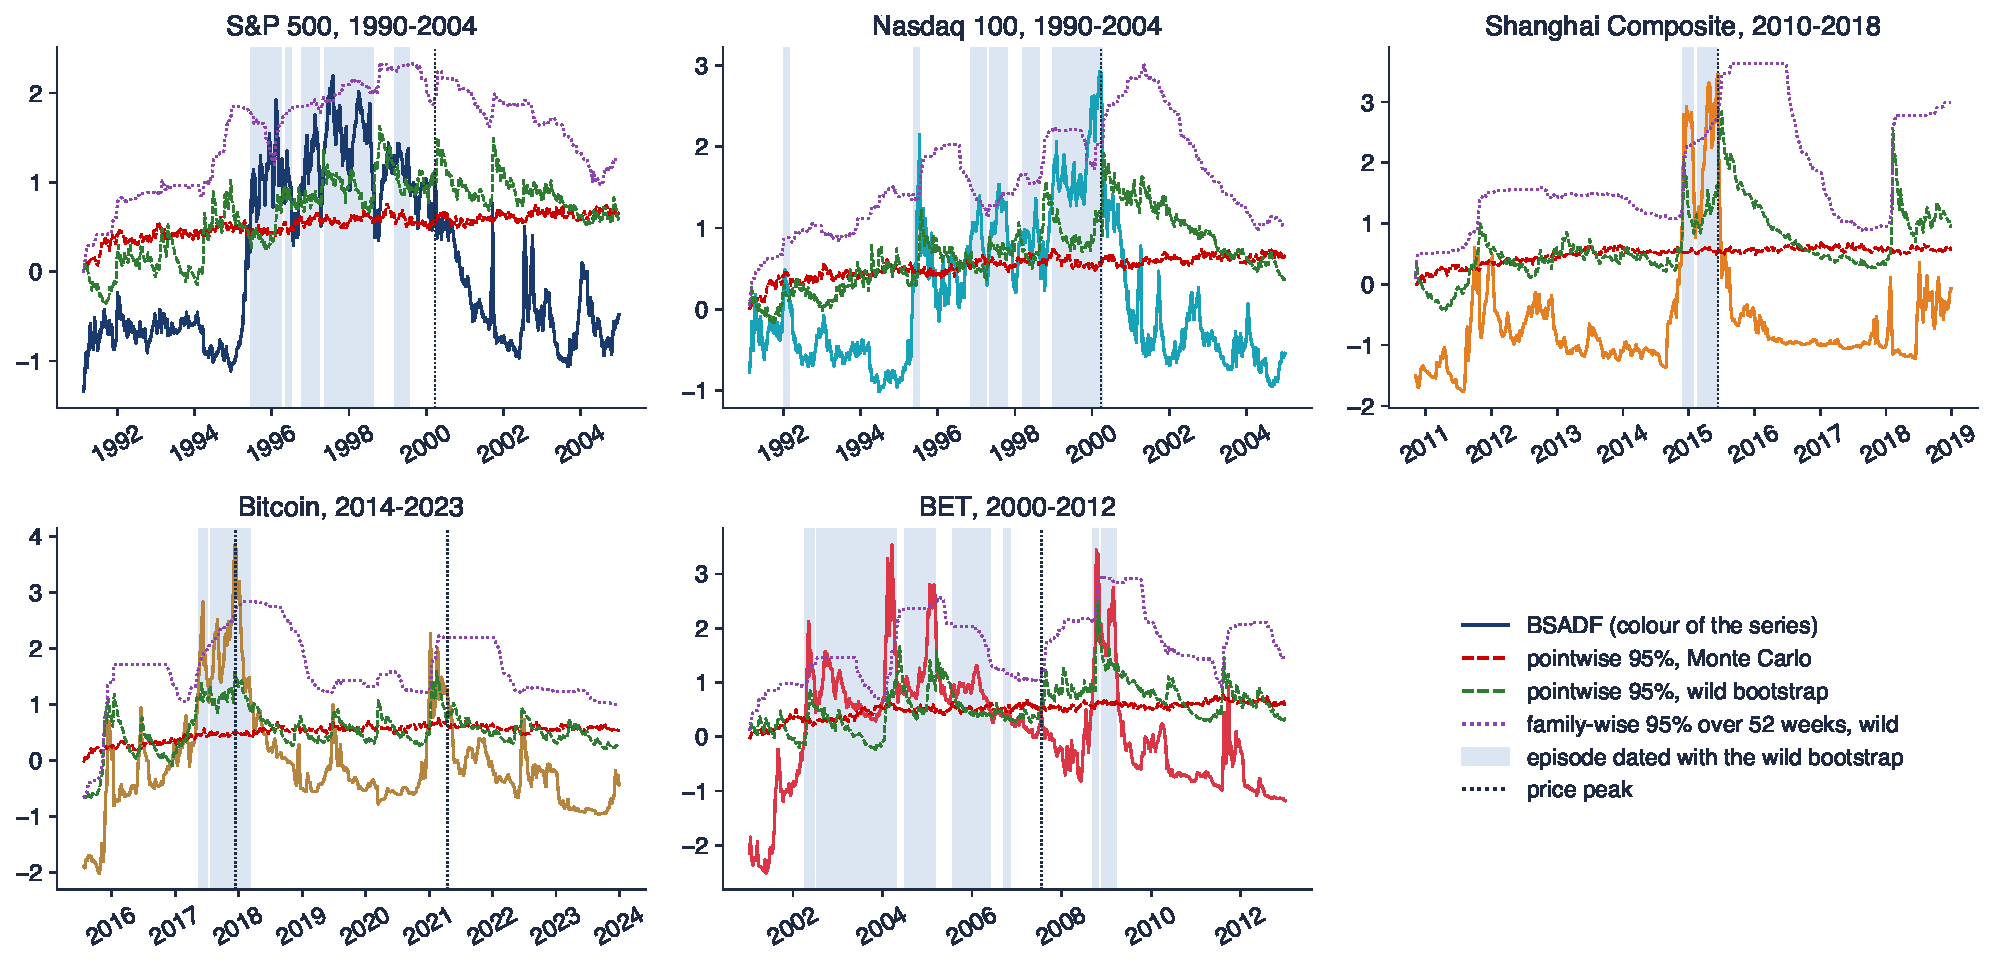
\includegraphics[width=0.97\textwidth,height=0.68\textheight,keepaspectratio]{ats_ch16_episodes.pdf}
\end{center}
\vspace{-0.25cm}
\begin{itemize}
    \item Shaded: episodes dated with the pointwise wild bootstrap; dotted vertical lines: price peaks
\end{itemize}
\quantlet{ATS\_ch16\_episodes}{\qlurl{ATS_ch16_episodes}}
\end{frame}

\begin{frame}{Interpreting the five tests}
\itemsize{\footnotesize}
\begin{center}
\scriptsize
\begin{tabular}{lrrrrrr}
\toprule
\textbf{Series} & $T$ & GSADF & \textbf{cv MC} & \textbf{cv wild} & \textbf{episodes: MC / wild / FW} & \textbf{weeks: MC / wild} \\
\midrule
S\&P 500 & 782 & 2.19 & 2.28 & 2.91 & 5 / 6 / 0 & 228 / 167 \\
Nasdaq 100 & 782 & 2.92 & 2.28 & 3.22 & 6 / 6 / 1 & 210 / 159 \\
Shanghai & 460 & 3.46 & 2.15 & 3.90 & 1 / 2 / 1 & 31 / 27 \\
Bitcoin & 484 & 3.85 & 2.18 & 3.15 & 2 / 2 / 1 & 75 / 43 \\
BET & 663 & 3.53 & 2.29 & 3.21 & 3 / 7 / 1 & 213 / 217 \\
\bottomrule
\end{tabular}
\end{center}
\begin{itemize}
    \item S\&P 500: GSADF below both critical values, yet pointwise dating marks 6 episodes: the multiplicity trap on real data; no family-wise episode
    \item The wild critical values exceed the Monte Carlo ones for every series (volatility clusters): Bitcoin and BET still reject; the Nasdaq (2.92 against 3.22) and Shanghai (3.46 against 3.90) do not
    \item MC: Monte Carlo; FW: family-wise wild threshold over 52 weeks; cv: 95\% critical value of GSADF
\end{itemize}
\end{frame}

\begin{frame}{Alarms before the peaks}
\itemsize{\footnotesize}
\begin{center}
\scriptsize
\begin{tabular}{lrrrrr}
\toprule
\textbf{Peak} & \textbf{first alarm (2 years before)} & \textbf{lead (weeks)} & \textbf{active at peak} & \textbf{FW lead} & \textbf{fall in 1 year} \\
\midrule
S\&P 500, 24 March 2000 & 16 April 1999 & 49 & no & -- & 25\% \\
Nasdaq 100, 24 March 2000 & 24 April 1998 & 100 & yes & 13 & 65\% \\
Shanghai, 12 June 2015 & 9 January 2015 & 22 & yes & 22 & 47\% \\
Bitcoin, 15 December 2017 & 23 June 2017 & 25 & yes & -- & 82\% \\
Bitcoin, 16 April 2021 & none & -- & no & -- & 49\% \\
BET, 20 July 2007 & 2 September 2005 & 98 & no & -- & 46\% \\
\bottomrule
\end{tabular}
\end{center}
\begin{itemize}
    \item Every major peak is preceded by a pointwise alarm except Bitcoin 2021; leads of half a year to two years: too early to time a crash, informative about the regime
    \item BET 2007: the alarm of 2 September 2005 is followed by almost two years of gains before the peak and a fall of 46\%; family-wise control removes most alarms
    \item Counting only peaks hides the false alarms: alarms that were not followed by a crash appear only when every date is evaluated
\end{itemize}
\end{frame}

\begin{frame}{Early-warning value over decades}
\itemsize{\footnotesize}
\begin{center}
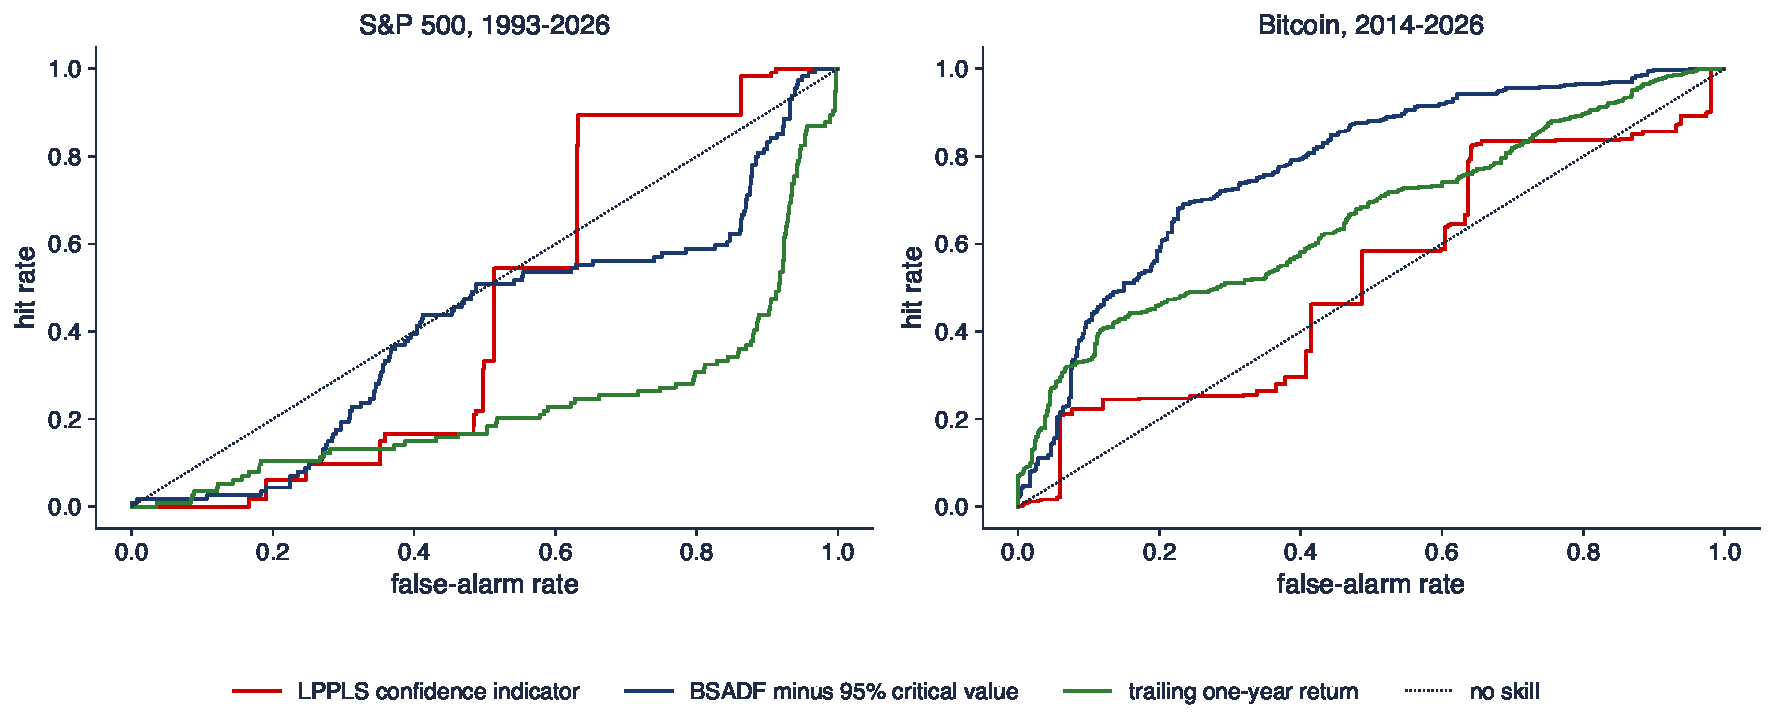
\includegraphics[width=0.97\textwidth,height=0.61\textheight,keepaspectratio]{ats_ch16_evaluation.pdf}
\end{center}
\vspace{-0.25cm}
\begin{itemize}
    \item Event: a fall of 20\% within 182 days; evaluation every fifth trading day (S\&P 500 1\,672 dates, Bitcoin 893); scores: LPPLS confidence indicator, BSADF minus its pointwise 95\% critical value (weekly, real time), trailing one-year return
\end{itemize}
\quantlet{ATS\_ch16\_early\_warning}{\qlurl{ATS_ch16_early_warning}}
\end{frame}

\begin{frame}{Interpreting the early-warning evaluation}
\itemsize{\footnotesize}
\begin{itemize}
    \item Base rates: 6.8\% of S\&P 500 dates and 47.6\% of Bitcoin dates are followed by a 20\% fall: the same alarm means very different things in the two markets
    \item S\&P 500, AUC with 90\% block-bootstrap intervals: indicator 0.39 [0.32, 0.48], BSADF 0.41 [0.28, 0.58], momentum 0.23 [0.10, 0.40]: all below 0.5
    \item Most S\&P 500 dates followed by a 20\% fall lie inside bear markets (2000--2002, 2008), when exuberance scores are low, and few at the top of a run-up
    \begin{itemize}
        \item so the scores are \textbf{lower} before the events; BSADF alarms have precision 1\% against a base rate of 6.8\%
    \end{itemize}
    \item Bitcoin: BSADF has skill, AUC 0.77 [0.69, 0.85], above momentum 0.66; its alarms reach precision 79\% against a base rate of 47.6\% (hit rate 32\%, false alarms 8\%)
    \item The LPPLS indicator is positive on 35.9\% of S\&P 500 dates and 4.6\% of Bitcoin dates; its AUC is 0.39 and 0.49: under this protocol it does not separate pre-crash dates from the rest
\end{itemize}
\end{frame}

\begin{frame}{Recap: the applications}
\itemsize{\small}
\begin{itemize}
    \item Wild-bootstrap critical values are higher than Monte Carlo ones on real data; some textbook rejections do not survive
    \item Major peaks are usually preceded by alarms, but with long and variable leads; family-wise control removes most of them
    \item Over decades, precision must be read against the base rate
    \begin{itemize}
        \item exuberance scores help for Bitcoin, where crashes follow run-ups
        \item they fail for the S\&P 500, where most pre-crash dates lie inside bear markets
    \end{itemize}
\end{itemize}
\end{frame}


%=============================================================================
\section{AI for scientific discovery}
%=============================================================================

\begin{frame}{An open question}
\itemsize{\small}
\begin{itemize}
    \item The question
    \begin{itemize}
        \item do explosive-root and LPPLS alarms carry information about large falls beyond momentum and volatility?
        \item once base rates, overlapping horizons and the search over assets are accounted for
    \end{itemize}
    \item A testable form
    \begin{itemize}
        \item formal: in a logit or probit of the event on lagged momentum, volatility and the alarm score, $H_0$: the alarm coefficient is zero, with block-bootstrap inference and a pre-registered panel of assets
        \item falsified by a significant out-of-sample gain in a proper score (log score, Brier) over the momentum-volatility model, pooled across assets
    \end{itemize}
    \item Why it matters
    \begin{itemize}
        \item regulators and investors read bubble indicators as warnings
        \item most evidence comes from a few famous episodes chosen after the fact
        \item literature to start from: \refPS, \refAHLST, \refDS, \refBJ, \refHB
    \end{itemize}
\end{itemize}
\end{frame}

\begin{frame}{The discovery loop with an AI assistant}
\itemsize{\footnotesize}
\begin{itemize}
    \item An AI assistant (an LLM such as Claude, ChatGPT, Gemini or Copilot) speeds up each step; Semantic Scholar and Elicit help with the literature
    \begin{itemize}
        \item \textbf{literature}: \aiprompt{List peer-reviewed papers since 2015 that evaluate bubble detectors out of sample with false-alarm rates; give DOIs.} Then check every DOI and the reported numbers
        \item \textbf{hypothesis}: \aiprompt{Write a pre-registration: assets, sample, event definition, scores, baseline model, proper score, test and block length.}
        \item \textbf{code and replication}: ask for a vectorised BSADF; reproduce a known number first (the GSADF of the Nasdaq 100 here, or PSY critical values)
        \item \textbf{critique}: \aiprompt{Act as a hostile referee: list every way this evaluation could overstate the value of the alarms.}
    \end{itemize}
    \item Report: what was asked, what was kept, what was rejected (AI\_USE.md, AI\_ERRORS.md)
\end{itemize}
\end{frame}

\begin{frame}{What the human checks}
\itemsize{\small}
\begin{itemize}
    \item Every reference exists and says what is claimed (DOI resolves, the title matches, the result is in the paper)
    \item Right tail, not left: an AI-written ADF often uses left-tail critical values or the 1.645 normal quantile
    \item Critical values simulated for the same $T$, $r_0$, lags and deterministic terms; wild bootstrap when volatility changes
    \item No look-ahead: the minimum window, the lag order and the scaling are fixed from data available at each date
    \item Multiplicity over dates and over assets: which error rate does a reported bubble control?
\end{itemize}
\end{frame}

\begin{frame}{Mini-case: how many bubbles does a screen find?}
\itemsize{\footnotesize}
\begin{center}
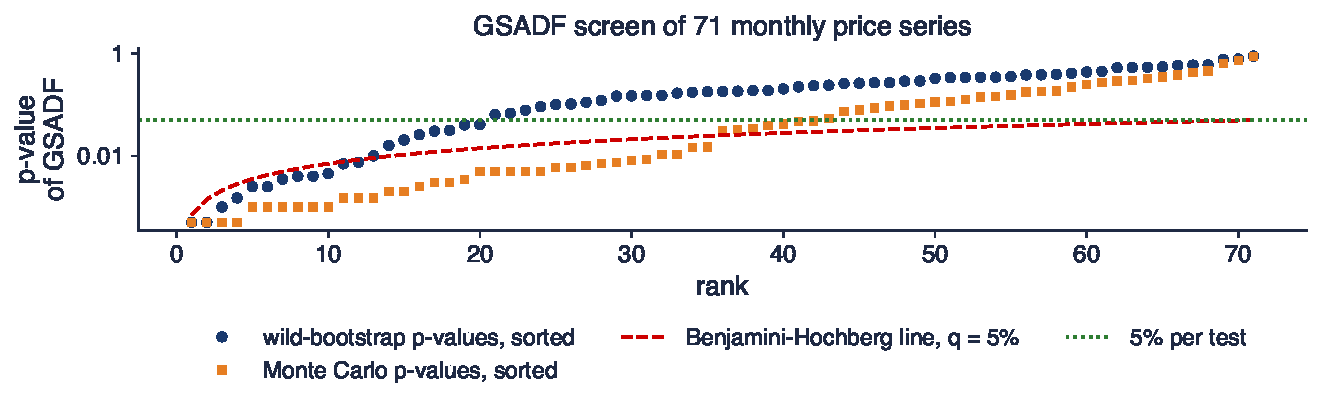
\includegraphics[width=0.97\textwidth,height=0.52\textheight,keepaspectratio]{ats_ch16_ai_case.pdf}
\end{center}
\vspace{-0.25cm}
\begin{itemize}
    \item GSADF on the monthly log price of 71 series of the course data (from 1990 or the first month), p-values from 1999 wild-bootstrap and 1999 Monte Carlo draws (smallest attainable p-value: 0.0005)
    \item Rejections at 5\%: 42 with Monte Carlo, 20 with the wild bootstrap (3.6 expected by chance); after Holm 2, after Benjamini--Hochberg 12. An AI summary such as \textquotedblleft bubbles in 42 assets\textquotedblright{} is wrong twice: wrong null and no correction
\end{itemize}
\quantlet{ATS\_ch16\_ai\_screen}{\qlurl{ATS_ch16_ai_screen}}
\end{frame}

\begin{frame}{Project idea}
\itemsize{\small}
\begin{itemize}
    \item \textbf{A pre-registered evaluation of bubble alarms on Central and Eastern European markets}
    \begin{itemize}
        \item replicate: the date-stamping of \refPSYa{} and the wild bootstrap with family-wise control of \refPS{} on BET, WIG20, BUX, PX and on housing price-to-rent ratios (Eurostat)
        \item extend: compare BSADF, monitoring with a boundary and the LPPLS indicator as predictors of 20\% falls, against momentum and volatility, with proper scores and block bootstrap
        \item pre-register: assets, event definition, scores, horizons, tests and the decision rule, before running anything after 1 November 2026
    \end{itemize}
    \item Deliverables follow the course rules: repository, report, AI\_USE.md, AI\_ERRORS.md, oral defence
\end{itemize}
\end{frame}


%=============================================================================
\section{Wrap-up}
%=============================================================================

\begin{frame}{Key takeaways}
\itemsize{\small}
\begin{itemize}
    \item A rational bubble is an explosive autoregressive component; it cannot be negative or start later, and periodic collapses hide it from whole-sample tests
    \item Explosive roots are learned at an exponential rate with Cauchy limits; mildly explosive asymptotics are invariant and justify the window tests
    \item Critical values must match the design; the wild bootstrap handles changing volatility; date-stamping needs family-wise control
    \item Dated starts are late, alarms are early relative to peaks, and precision depends on the base rate
    \item Test fundamentals as well as prices; judge LPPLS and PSY by the same alarms, events and scores
\end{itemize}
\end{frame}

\begin{frame}{Key formulas}
\itemsize{\small}
{\renewcommand{\arraystretch}{1.4}\begin{center}
\footnotesize
\begin{tabular}{ll}
\toprule
\textbf{Object} & \textbf{Formula} \\
\midrule
Bubble & $P_t = F_t + B_t$, $\E_t B_{t+1} = (1 + r)B_t$ \\
Fundamental, random-walk dividends & $F_t = D_t/r + \mu(1 + r)/r^2$ \\
Explosive OLS limit & $\rho^n(\hat\rho - \rho)/(\rho^2 - 1) \Rightarrow \mathcal C$ \\
Recursive statistics & $\mathrm{BSADF}_{r_2} = \sup_{r_1}\mathrm{ADF}_{r_1}^{r_2}$, $\mathrm{GSADF} = \sup_{r_2}\mathrm{BSADF}_{r_2}$ \\
Minimum window & $r_0 = 0.01 + 1.8/\sqrt T$ \\
Monitoring boundary & $b_t = \sqrt{\tfrac{t - n}{n}\tfrac{t}{n}[a^2 + \ln\tfrac{t}{t - n}]}$, $1 - \Phi(a) + a\varphi(a) = \alpha$ \\
Precision of an alarm & $H\pi_0/[H\pi_0 + F(1 - \pi_0)]$ \\
LPPLS & $\ln p = A + B f + C_1 f\cos(\omega\ln(t_c - t)) + C_2 f\sin(\omega\ln(t_c - t))$, $f = (t_c - t)^m$ \\
\bottomrule
\end{tabular}
\end{center}
}
\end{frame}

\begin{frame}{Self-assessment (1/2)}
\itemsize{\small}
\begin{itemize}
    \item Derive $F_t$ when dividends follow $D_t = \mu + D_{t-1} + \varepsilon_t$; what is $F_t$ for $r = 0.04$, $\mu = 0.1$, $D_t = 3$?
    \item Why can a rational bubble not start after the first trading day?
    \item Why does the whole-sample ADF fail against an Evans bubble?
    \item Why is the limit of $\hat\rho$ for a fixed explosive root Cauchy only with Gaussian errors?
    \item A sample has $T = 400$ weeks. What are $r_0$ and the minimum window?
    \item Why is the GSADF critical value larger than the SADF one?
\end{itemize}
\end{frame}

\begin{frame}{Self-assessment (2/2)}
\itemsize{\small}
\begin{itemize}
    \item What does the wild bootstrap keep from the data, and what does it remove?
    \item An alarm has $H = 0.7$ and $F = 0.1$; the base rate is 4\%. What is its precision?
    \item Why must the alarm date be the confirmation date and not the dated start?
    \item The price-to-rent ratio is explosive and real rents are explosive too. What do you conclude?
    \item Why is a profile-likelihood interval for $t_c$ too narrow with autocorrelated residuals?
    \item A screen of 80 assets finds 20 GSADF rejections at 5\%. Which two checks come first?
\end{itemize}
\end{frame}

\begin{frame}{Self-assessment: answers (1/2)}
\itemsize{\small}
\begin{itemize}
    \item $F_t = D_t/r + \mu(1 + r)/r^2 = 75 + 65 = 140$
    \item If $B_t = 0$, then $\E_t B_{t+1} = 0$ and $B_{t+1} \ge 0$ (no negative bubbles), so $B_{t+1} = 0$ almost surely; by induction the bubble stays at zero
    \item Collapses pair the largest falls with the highest levels and pull the OLS slope down; over the whole sample the series looks I(1) or stationary
    \item $\rho^n(\hat\rho - \rho)/(\rho^2 - 1) \approx X_n/Y_n$ with $X_n$, $Y_n$ dominated by a few shocks: they are normal only if the shocks are normal; no CLT acts inside them
    \item $r_0 = 0.01 + 1.8/20 = 0.1$; minimum window $\lfloor 0.1 \cdot 400\rfloor = 40$ weeks
    \item GSADF takes a supremum over more windows (all starts and ends), so under the null its maximum is larger
\end{itemize}
\end{frame}

\begin{frame}{Self-assessment: answers (2/2)}
\itemsize{\small}
\begin{itemize}
    \item It keeps the volatility pattern $|\hat e_t|$ (and the short-run dynamics of the null model); random signs remove any explosive or predictable component
    \item $0.7 \cdot 0.04/(0.7 \cdot 0.04 + 0.1 \cdot 0.96) = 0.028/0.124 \approx 0.23$
    \item The start is known only after the minimum number of exceedances; using it as the alarm date would use future information
    \item No evidence of a bubble from these tests: the fundamental explains the acceleration; one would test whether the ratio explodes beyond what rents imply
    \item Autocorrelated residuals carry less information than $n$ independent errors, and nuisance parameters are ignored: the likelihood is too sharp
    \item Whether the critical values allow for changing volatility (wild bootstrap); whether the number of rejections survives a multiple-testing correction (4 are expected by chance)
\end{itemize}
\end{frame}

\begin{frame}{Further reading and links}
\itemsize{\small}
\begin{columns}[T]
\begin{column}{0.34\textwidth}
\centering
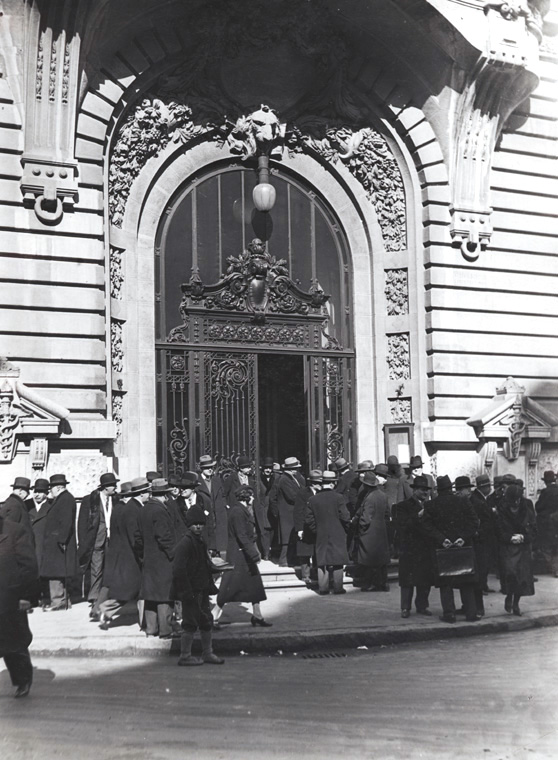
\includegraphics[height=0.4\textheight]{ch16_bvb_palace_1928.jpg}\\[1mm]
\imgcap{The Bucharest Stock Exchange Palace, March 1928}
\imgcredit{https://commons.wikimedia.org/wiki/File:Nicolae_Ionescu_-_The_Stock_Exchange_Palace_in_March_1928.jpg}{Photo: Nicolae Ionescu (1928); public domain; Wikimedia Commons}
\end{column}
\begin{column}{0.64\textwidth}
\begin{itemize}
    \item Surveys
    \begin{itemize}
        \item \refGur; \refShi; \refKA
        \item bubbles and later returns: \refGSY
    \end{itemize}
    \item Implementation: the R package \texttt{exuber} \refVPM
    \begin{itemize}
        \item our Quantlets reproduce its statistics in Python
    \end{itemize}
    \item Applications to markets, risk and policy: \atschlink{https://danpele.github.io/MFM/EN/Courses/chapter17_bubbles_crashes.pdf}{MFM, Chapter 17}
    \item Further reading on the Bucharest Stock Exchange: \refPMM
    \item The course ends here; the project defence is described in \atschlink{https://danpele.github.io/Advanced-Time-Series/EN/Courses/chapter15_review_project_defence.pdf}{Chapter 15}
\end{itemize}
\end{column}
\end{columns}
\end{frame}


%=============================================================================
\section{Appendix}
%=============================================================================

\begin{frame}{Appendix: the mildly explosive Cauchy limit}
\hypertarget{atsapp1}{}\atsappback{atssrc1}{Back}
\itemsize{\small}
\begin{itemize}
    \item $\rho_n = 1 + c/k_n$; $X_n = k_n^{-1/2}\sum_{j=1}^{n}\rho_n^{-(n-j)-1}u_j$, $Y_n = k_n^{-1/2}\sum_{j=1}^{n}\rho_n^{-j}u_j$; weights $\rho_n^{-j} \approx e^{-cj/k_n}$ decay over $O(k_n)$ terms
    \item Lindeberg: no single weight dominates, so $(X_n, Y_n) \Rightarrow (X, Y)$, independent $N(0, \sigma^2/2c)$ ($\sum_j\rho_n^{-2j} \approx k_n/2c$); independence because $X_n$ and $Y_n$ load on the two ends of the sample and $k_n = o(n)$
    \item $(k_n\rho_n^n)^{-2}\sum_t y_{t-1}^2 \Rightarrow Y^2/2c$ and $(k_n\rho_n^n)^{-1}\sum_t y_{t-1}u_t \Rightarrow XY$, so $\dfrac{k_n\rho_n^n}{2c}(\hat\rho - \rho_n) \Rightarrow X/Y \sim \mathcal C$ \refPM
    \item A ratio of two independent centred normals with equal variances is standard Cauchy: $X/Y = \tan\Theta$ with $\Theta$ uniform on $(-\pi/2, \pi/2)$
\end{itemize}
\end{frame}

\begin{frame}{Appendix: the monitoring boundary}
\hypertarget{atsapp2}{}\atsappback{atssrc2}{Back}
\itemsize{\small}
\begin{itemize}
    \item Under the null, $S_t \approx n^{-1/2}\sigma^{-1}[\sum_{j \le t}\varepsilon_j - (t/n)\sum_{j \le n}\varepsilon_j]$; with $s = (t - n)/n$: $S \Rightarrow Z(s) = W(1 + s) - (1 + s)W(1)$, $\Var Z(s) = s(1 + s)$
    \item Time inversion: $Z(s) = s\,B(1 + 1/s)$ for a standard Brownian motion $B$; with $u = 1/s$ the event $Z(s) > \sqrt{s(1 + s)[a^2 + \ln((1 + s)/s)]}$ becomes $B(1 + u) > \sqrt{(1 + u)[a^2 + \ln(1 + u)]}$
    \item Robbins--Siegmund: $\Pr\{B(1 + u) > \sqrt{(1 + u)[a^2 + \ln(1 + u)]}$ for some $u \ge 0\} = 1 - \Phi(a) + a\varphi(a)$; the two-sided version doubles it, the form used by \refCSW
    \item In $t$: $s(1 + s) = \frac{t - n}{n}\cdot\frac{t}{n}$ and $(1 + s)/s = t/(t - n)$, which gives $b_t$; a finite horizon makes the test conservative
\end{itemize}
\end{frame}


%=============================================================================
\section{References}
%=============================================================================

\begin{frame}{References (1/4)}
\itemsize{\tiny}
\begin{itemize}
    \item Anderson, T. W. (1959). On asymptotic distributions of estimates of parameters of stochastic difference equations. \textit{The Annals of Mathematical Statistics}, 30(3), 676--687. \href{https://doi.org/10.1214/aoms/1177706198}{doi:10.1214/aoms/1177706198}
    \item Astill, S., Harvey, D. I., Leybourne, S. J., Sollis, R., \& Taylor, A. M. R. (2018). Real-time monitoring for explosive financial bubbles. \textit{Journal of Time Series Analysis}, 39(6), 863--891. \href{https://doi.org/10.1111/jtsa.12409}{doi:10.1111/jtsa.12409}
    \item Astill, S., Harvey, D. I., Leybourne, S. J., \& Taylor, A. M. R. (2017). Tests for an end-of-sample bubble in financial time series. \textit{Econometric Reviews}, 36(6--9), 651--666. \href{https://doi.org/10.1080/07474938.2017.1307490}{doi:10.1080/07474938.2017.1307490}
    \item Blanchard, O. J., \& Watson, M. W. (1982). Bubbles, rational expectations and financial markets. NBER Working Paper 945. \href{https://doi.org/10.3386/w0945}{doi:10.3386/w0945}
    \item Brée, D. S., \& Joseph, N. L. (2013). Testing for financial crashes using the log periodic power law model. \textit{International Review of Financial Analysis}, 30, 287--297. \href{https://doi.org/10.1016/j.irfa.2013.05.005}{doi:10.1016/j.irfa.2013.05.005}
    \item Campbell, J. Y., \& Shiller, R. J. (1987). Cointegration and tests of present value models. \textit{Journal of Political Economy}, 95(5), 1062--1088. \href{https://doi.org/10.1086/261502}{doi:10.1086/261502}
    \item Chu, C.-S. J., Stinchcombe, M., \& White, H. (1996). Monitoring structural change. \textit{Econometrica}, 64(5), 1045--1065. \href{https://doi.org/10.2307/2171955}{doi:10.2307/2171955}
    \item Demos, G., \& Sornette, D. (2017). Birth or burst of financial bubbles: Which one is easier to diagnose? \textit{Quantitative Finance}, 17(5), 657--675. \href{https://doi.org/10.1080/14697688.2016.1231417}{doi:10.1080/14697688.2016.1231417}
    \item Diba, B. T., \& Grossman, H. I. (1988a). The theory of rational bubbles in stock prices. \textit{The Economic Journal}, 98(392), 746--754. \href{https://doi.org/10.2307/2233912}{doi:10.2307/2233912}
    \item Diba, B. T., \& Grossman, H. I. (1988b). Explosive rational bubbles in stock prices? \textit{American Economic Review}, 78(3), 520--530. \href{https://ideas.repec.org/a/aea/aecrev/v78y1988i3p520-30.html}{ideas.repec.org}
    \item Dickey, D. A., \& Fuller, W. A. (1979). Distribution of the estimators for autoregressive time series with a unit root. \textit{Journal of the American Statistical Association}, 74(366), 427--431. \href{https://doi.org/10.1080/01621459.1979.10482531}{doi:10.1080/01621459.1979.10482531}
    \item Evans, G. W. (1991). Pitfalls in testing for explosive bubbles in asset prices. \textit{American Economic Review}, 81(4), 922--930. \href{https://ideas.repec.org/a/aea/aecrev/v81y1991i4p922-30.html}{ideas.repec.org}
\end{itemize}
\end{frame}

\begin{frame}{References (2/4)}
\itemsize{\tiny}
\begin{itemize}
    \item Feigenbaum, J. A. (2001). A statistical analysis of log-periodic precursors to financial crashes. \textit{Quantitative Finance}, 1(3), 346--360. \href{https://doi.org/10.1088/1469-7688/1/3/306}{doi:10.1088/1469-7688/1/3/306}
    \item Filimonov, V., Demos, G., \& Sornette, D. (2017). Modified profile likelihood inference and interval forecast of the burst of financial bubbles. \textit{Quantitative Finance}, 17(8), 1167--1186. \href{https://doi.org/10.1080/14697688.2016.1276298}{doi:10.1080/14697688.2016.1276298}
    \item Filimonov, V., \& Sornette, D. (2013). A stable and robust calibration scheme of the log-periodic power law model. \textit{Physica A}, 392(17), 3698--3707. \href{https://doi.org/10.1016/j.physa.2013.04.012}{doi:10.1016/j.physa.2013.04.012}
    \item Geraskin, P., \& Fantazzini, D. (2013). Everything you always wanted to know about log-periodic power laws for bubble modeling but were afraid to ask. \textit{The European Journal of Finance}, 19(5), 366--391. \href{https://doi.org/10.1080/1351847X.2011.601657}{doi:10.1080/1351847X.2011.601657}
    \item Gerlach, J.-C., Demos, G., \& Sornette, D. (2019). Dissection of Bitcoin\textquoteright s multiscale bubble history from January 2012 to February 2018. \textit{Royal Society Open Science}, 6(7), 180643. \href{https://doi.org/10.1098/rsos.180643}{doi:10.1098/rsos.180643}
    \item Greenwood, R., Shleifer, A., \& You, Y. (2019). Bubbles for Fama. \textit{Journal of Financial Economics}, 131(1), 20--43. \href{https://doi.org/10.1016/j.jfineco.2018.09.002}{doi:10.1016/j.jfineco.2018.09.002}
    \item Gürkaynak, R. S. (2008). Econometric tests of asset price bubbles: Taking stock. \textit{Journal of Economic Surveys}, 22(1), 166--186. \href{https://doi.org/10.1111/j.1467-6419.2007.00530.x}{doi:10.1111/j.1467-6419.2007.00530.x}
    \item Hamilton, J. D. (1994). \textit{Time Series Analysis}. Princeton University Press. \href{https://doi.org/10.1515/9780691218632}{doi:10.1515/9780691218632}
    \item Harvey, D. I., Leybourne, S. J., \& Sollis, R. (2017). Improving the accuracy of asset price bubble start and end date estimators. \textit{Journal of Empirical Finance}, 40, 121--138. \href{https://doi.org/10.1016/j.jempfin.2016.11.001}{doi:10.1016/j.jempfin.2016.11.001}
    \item Harvey, D. I., Leybourne, S. J., Sollis, R., \& Taylor, A. M. R. (2016). Tests for explosive financial bubbles in the presence of non-stationary volatility. \textit{Journal of Empirical Finance}, 38, 548--574. \href{https://doi.org/10.1016/j.jempfin.2015.09.002}{doi:10.1016/j.jempfin.2015.09.002}
    \item Harvey, D. I., Leybourne, S. J., \& Zu, Y. (2020). Sign-based unit root tests for explosive financial bubbles in the presence of deterministically time-varying volatility. \textit{Econometric Theory}, 36(1), 122--169. \href{https://doi.org/10.1017/S0266466619000057}{doi:10.1017/S0266466619000057}
    \item Homm, U., \& Breitung, J. (2012). Testing for speculative bubbles in stock markets: A comparison of alternative methods. \textit{Journal of Financial Econometrics}, 10(1), 198--231. \href{https://doi.org/10.1093/jjfinec/nbr009}{doi:10.1093/jjfinec/nbr009}
\end{itemize}
\end{frame}

\begin{frame}{References (3/4)}
\itemsize{\tiny}
\begin{itemize}
    \item Johansen, A., Ledoit, O., \& Sornette, D. (2000). Crashes as critical points. \textit{International Journal of Theoretical and Applied Finance}, 3(2), 219--255. \href{https://doi.org/10.1142/S0219024900000115}{doi:10.1142/S0219024900000115}
    \item Kaminsky, G., Lizondo, S., \& Reinhart, C. M. (1998). Leading indicators of currency crises. \textit{IMF Staff Papers}, 45(1), 1--48. \href{https://doi.org/10.2307/3867328}{doi:10.2307/3867328}
    \item Kindleberger, C. P., \& Aliber, R. Z. (2005). \textit{Manias, Panics and Crashes: A History of Financial Crises} (5th ed.). Palgrave Macmillan. \href{https://doi.org/10.1057/9780230628045}{doi:10.1057/9780230628045}
    \item Lomb, N. R. (1976). Least-squares frequency analysis of unequally spaced data. \textit{Astrophysics and Space Science}, 39(2), 447--462. \href{https://doi.org/10.1007/BF00648343}{doi:10.1007/BF00648343}
    \item Pavlidis, E., Yusupova, A., Paya, I., Peel, D., Martínez-García, E., Mack, A., \& Grossman, V. (2016). Episodes of exuberance in housing markets: In search of the smoking gun. \textit{The Journal of Real Estate Finance and Economics}, 53(4), 419--449. \href{https://doi.org/10.1007/s11146-015-9531-2}{doi:10.1007/s11146-015-9531-2}
    \item Pele, D. T., \& Mazurencu-Marinescu, M. (2012). Modelling stock market crashes: The case of Bucharest Stock Exchange. \textit{Procedia -- Social and Behavioral Sciences}, 58, 533--542 (further reading). \href{https://doi.org/10.1016/j.sbspro.2012.09.1030}{doi:10.1016/j.sbspro.2012.09.1030}
    \item Phillips, P. C. B., \& Magdalinos, T. (2007). Limit theory for moderate deviations from a unit root. \textit{Journal of Econometrics}, 136(1), 115--130. \href{https://doi.org/10.1016/j.jeconom.2005.08.002}{doi:10.1016/j.jeconom.2005.08.002}
    \item Phillips, P. C. B., \& Shi, S. (2018). Financial bubble implosion and reverse regression. \textit{Econometric Theory}, 34(4), 705--753. \href{https://doi.org/10.1017/S0266466617000202}{doi:10.1017/S0266466617000202}
    \item Phillips, P. C. B., \& Shi, S. (2020). Real time monitoring of asset markets: Bubbles and crises. In \textit{Handbook of Statistics}, Vol.\ 42, 61--80. Elsevier. \href{https://doi.org/10.1016/bs.host.2018.12.002}{doi:10.1016/bs.host.2018.12.002}
    \item Phillips, P. C. B., Shi, S., \& Yu, J. (2015a). Testing for multiple bubbles: Historical episodes of exuberance and collapse in the S\&P 500. \textit{International Economic Review}, 56(4), 1043--1078. \href{https://doi.org/10.1111/iere.12132}{doi:10.1111/iere.12132}
    \item Phillips, P. C. B., Shi, S., \& Yu, J. (2015b). Testing for multiple bubbles: Limit theory of real-time detectors. \textit{International Economic Review}, 56(4), 1079--1134. \href{https://doi.org/10.1111/iere.12131}{doi:10.1111/iere.12131}
    \item Phillips, P. C. B., Shi, S., \& Yu, J. (2014). Specification sensitivity in right-tailed unit root testing for explosive behaviour. \textit{Oxford Bulletin of Economics and Statistics}, 76(3), 315--333. \href{https://doi.org/10.1111/obes.12026}{doi:10.1111/obes.12026}
\end{itemize}
\end{frame}

\begin{frame}{References (4/4)}
\itemsize{\tiny}
\begin{itemize}
    \item Phillips, P. C. B., Wu, Y., \& Yu, J. (2011). Explosive behavior in the 1990s Nasdaq: When did exuberance escalate asset values? \textit{International Economic Review}, 52(1), 201--226. \href{https://doi.org/10.1111/j.1468-2354.2010.00625.x}{doi:10.1111/j.1468-2354.2010.00625.x}
    \item Phillips, P. C. B., \& Yu, J. (2011). Dating the timeline of financial bubbles during the subprime crisis. \textit{Quantitative Economics}, 2(3), 455--491. \href{https://doi.org/10.3982/QE82}{doi:10.3982/QE82}
    \item Santos, M. S., \& Woodford, M. (1997). Rational asset pricing bubbles. \textit{Econometrica}, 65(1), 19--57. \href{https://doi.org/10.2307/2171812}{doi:10.2307/2171812}
    \item Shiller, R. J. (2015). \textit{Irrational Exuberance} (3rd ed.). Princeton University Press. \href{https://doi.org/10.1515/9781400865536}{doi:10.1515/9781400865536}
    \item Shu, M., \& Zhu, W. (2020). Detection of Chinese stock market bubbles with LPPLS confidence indicator. \textit{Physica A}, 557, 124892. \href{https://doi.org/10.1016/j.physa.2020.124892}{doi:10.1016/j.physa.2020.124892}
    \item Sornette, D., Demos, G., Zhang, Q., Cauwels, P., \& Zhang, Q. (2015). Real-time prediction and post-mortem analysis of the Shanghai 2015 stock market bubble and crash. \textit{Journal of Investment Strategies}, 4(4), 77--95. \href{https://doi.org/10.21314/JOIS.2015.063}{doi:10.21314/JOIS.2015.063}
    \item Sornette, D., Woodard, R., Yan, W., \& Zhou, W.-X. (2013). Clarifications to questions and criticisms on the Johansen--Ledoit--Sornette financial bubble model. \textit{Physica A}, 392(19), 4417--4428. \href{https://doi.org/10.1016/j.physa.2013.05.011}{doi:10.1016/j.physa.2013.05.011}
    \item Tirole, J. (1985). Asset bubbles and overlapping generations. \textit{Econometrica}, 53(6), 1499--1528. \href{https://doi.org/10.2307/1913232}{doi:10.2307/1913232}
    \item Vasilopoulos, K., Pavlidis, E., \& Martínez-García, E. (2022). exuber: Recursive right-tailed unit root testing with R. \textit{Journal of Statistical Software}, 103(10). \href{https://doi.org/10.18637/jss.v103.i10}{doi:10.18637/jss.v103.i10}
    \item White, J. S. (1958). The limiting distribution of the serial correlation coefficient in the explosive case. \textit{The Annals of Mathematical Statistics}, 29(4), 1188--1197. \href{https://doi.org/10.1214/aoms/1177706450}{doi:10.1214/aoms/1177706450}
    \item Zhou, W.-X., \& Sornette, D. (2003). Nonparametric analyses of log-periodic precursors to financial crashes. \textit{International Journal of Modern Physics C}, 14(8), 1107--1125. \href{https://doi.org/10.1142/S0129183103005212}{doi:10.1142/S0129183103005212}
\end{itemize}
\end{frame}

\end{document}
